\documentclass[11pt,a4paper]{article}
\usepackage[utf8]{inputenc}
\usepackage[margin=2.4cm]{geometry}
\usepackage{amsmath,amssymb,amsthm,mathtools,bm}
\usepackage{booktabs,array,xcolor,enumitem,microtype}
\usepackage{float}
\usepackage[colorlinks=true,linkcolor=blue!50!black,urlcolor=blue!50!black]{hyperref}
\usepackage{tikz,pgfplots}
\usetikzlibrary{arrows.meta,calc,positioning,shapes.geometric,shapes.symbols,decorations.pathreplacing,fit,backgrounds}
\usepgfplotslibrary{groupplots}
\pgfplotsset{compat=1.16}
\usepackage[most]{tcolorbox}
\setlist{itemsep=2pt,topsep=3pt}
\setlength{\parindent}{0pt}
\setlength{\parskip}{5pt}

% ---------- notation ----------
\newcommand{\R}{\mathbb{R}}
\newcommand{\E}{\mathbb{E}}
\newcommand{\xx}{\boldsymbol{x}}
\newcommand{\om}{\boldsymbol{\omega}}
\newcommand{\cc}{\boldsymbol{c}}
\newcommand{\dd}{\boldsymbol{d}}
\newcommand{\Le}{L_e}
\newcommand{\dif}{\,\mathrm{d}}
\newcommand{\sref}[1]{\texorpdfstring{\emph{(slides #1)}}{(slides #1)}}

% ---------- theorem-like boxes ----------
\theoremstyle{definition}
\newtheorem{definition}{Definition}[section]
\newtheorem{example}{Example}[section]
\newtheorem{algorithm}{Algorithm}[section]
\theoremstyle{plain}
\newtheorem{lemma}{Lemma}[section]
\newtheorem{theorem}{Theorem}[section]
\newtheorem{proposition}{Proposition}[section]
\newtheorem{corollary}{Corollary}[section]
\tcolorboxenvironment{definition}{enhanced,breakable,colback=gray!6,colframe=gray!60!black,boxrule=0.6pt,sharp corners,left=5pt,right=5pt,top=3pt,bottom=3pt,before skip=8pt,after skip=8pt}
\tcolorboxenvironment{example}{enhanced,breakable,colback=green!4,colframe=green!45!black,boxrule=0.6pt,sharp corners,left=5pt,right=5pt,top=3pt,bottom=3pt,before skip=8pt,after skip=8pt}
\tcolorboxenvironment{algorithm}{enhanced,breakable,colback=violet!4,colframe=violet!60!black,boxrule=0.6pt,sharp corners,left=5pt,right=5pt,top=3pt,bottom=3pt,before skip=8pt,after skip=8pt}
\tcolorboxenvironment{lemma}{enhanced,breakable,colback=orange!5,colframe=orange!70!black,boxrule=0.6pt,sharp corners,left=5pt,right=5pt,top=3pt,bottom=3pt,before skip=8pt,after skip=8pt}
\tcolorboxenvironment{theorem}{enhanced,breakable,colback=orange!5,colframe=orange!70!black,boxrule=0.6pt,sharp corners,left=5pt,right=5pt,top=3pt,bottom=3pt,before skip=8pt,after skip=8pt}
\tcolorboxenvironment{proposition}{enhanced,breakable,colback=orange!5,colframe=orange!70!black,boxrule=0.6pt,sharp corners,left=5pt,right=5pt,top=3pt,bottom=3pt,before skip=8pt,after skip=8pt}
\tcolorboxenvironment{corollary}{enhanced,breakable,colback=orange!5,colframe=orange!70!black,boxrule=0.6pt,sharp corners,left=5pt,right=5pt,top=3pt,bottom=3pt,before skip=8pt,after skip=8pt}

\newtcolorbox{intuition}{enhanced,breakable,colback=blue!6,colframe=blue!55!black,
  title={Intuition},fonttitle=\bfseries\small,boxrule=0.6pt,arc=2pt,left=6pt,right=6pt,top=3pt,bottom=3pt,
  before skip=6pt,after skip=10pt}

% placeholder for photos / screenshots to be pasted from the slides
\newcommand{\slideimg}[3]{% #1 slide(s), #2 height, #3 caption
\begin{figure}[H]
\centering
\begin{tcolorbox}[enhanced,colback=white,colframe=white,boxrule=0pt,sharp corners,overlay={\draw[dashed,gray,thick] (frame.south west) rectangle (frame.north east);},
  width=0.92\linewidth,height=#2,valign=center,halign=center]
{\color{gray}\itshape Insert image here --- take it from slide #1}
\end{tcolorbox}
\caption{#3}
\end{figure}}

\title{\textbf{Foundations of Spatial AI}\\[2pt] Lecture 08 --- Neural Radiance Fields\\[2pt]\large Detailed lecture notes}
\author{Based on the slides by Emanuele Giacomini, Sapienza University of Rome (October 18, 2026)}
\date{}

\begin{document}
\maketitle
\begin{abstract}\small
These notes follow the flow of the lecture slides: we recall \emph{computational volume rendering} (ray marching), then ask how a volume can be \emph{represented} so that density and emitted light can be queried at any 3D point --- a voxel grid, an MLP (the Neural Radiance Field), voxels with spherical-harmonic colours (Plenoxels) and finally feature hash-grids with a tiny MLP (Instant-NGP). Along the way we discuss positional encoding, hierarchical and inverse-depth sampling, view-dependent effects and anti-aliasing (mip-NeRF). Slide ranges are given in each section title. No companion book chapter was provided, so the formal statements (definitions, lemmas, proofs) were derived from the slides and from the cited papers (NeRF, Fourier Features, mip-NeRF, Plenoxels, Instant-NGP).
\end{abstract}
\tableofcontents
\newpage

%==============================================================
\section{Neural Radiance Fields \sref{1--2}}
%==============================================================

The goal of the lecture is summarised in one line on slide~2:
\[
\text{posed images}\;\longrightarrow\;\text{a neural network}\;\longrightarrow\;\text{novel views.}
\]

\begin{figure}[H]
\centering
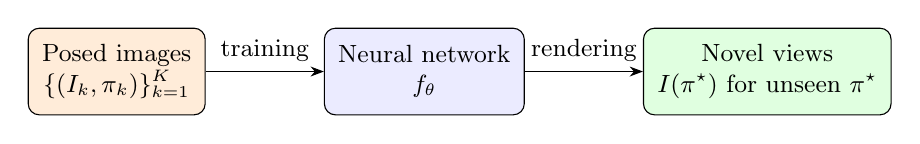
\begin{tikzpicture}[every node/.style={font=\small},
 box/.style={draw,rounded corners,minimum height=1.1cm,align=center,fill=blue!8,inner sep=5pt}]
\node[box,fill=orange!15] (img) {Posed images\\ $\{(I_k,\pi_k)\}_{k=1}^{K}$};
\node[box,right=1.5cm of img] (net) {Neural network\\ $f_\theta$};
\node[box,fill=green!12,right=1.5cm of net] (nv) {Novel views\\ $I(\pi^\star)$ for unseen $\pi^\star$};
\draw[-{Stealth}] (img)--(net) node[midway,above]{training};
\draw[-{Stealth}] (net)--(nv) node[midway,above]{rendering};
\end{tikzpicture}
\caption{The NeRF problem at a glance (redrawn from slide 2): learn $f_\theta$ from images with known cameras $\pi_k$, then render images from cameras never seen during training.}
\end{figure}

\slideimg{2}{5cm}{Left: nine of the posed training images of the NeRF ``lego'' scene; right: a novel view rendered by \texttt{nerfacto} (Nerfstudio). Figure credits: Mildenhall et al., ECCV 2020 (NeRF).}

\begin{definition}[Novel-view synthesis]
Given images $I_1,\dots,I_K$ of a static scene together with their camera parameters $\pi_1,\dots,\pi_K$ (intrinsics and pose), \emph{novel-view synthesis} (NVS) is the task of producing the image $I(\pi^\star)$ that a camera with parameters $\pi^\star\notin\{\pi_k\}$ would see.
\end{definition}

\begin{definition}[Radiance field]
A \emph{radiance field} is a function $(\xx,\om)\mapsto(\sigma,\cc)$ that assigns to every 3D point $\xx\in\R^3$ and viewing direction $\om\in\mathbb{S}^2$ a volume density $\sigma\in\R^+$ and an emitted colour (radiance) $\cc\in[0,1]^3$. A \emph{Neural} Radiance Field (NeRF) is a radiance field parameterised by a neural network $f_\theta$.
\end{definition}

\begin{intuition}
Think of the scene as a cloud of coloured, glowing smoke. $\sigma(\xx)$ says ``how thick is the smoke here?'' and $\cc(\xx,\om)$ says ``what colour does it glow when seen from direction $\om$?''. A photograph is what you get by looking at this cloud through a pinhole. Training means adjusting the cloud until all the photographs we have are reproduced; because the cloud is a genuine 3D object, we can then look at it from anywhere.
\end{intuition}

\textbf{Roadmap of the lecture.} The method has two ingredients that the slides keep separate:
(i)~a \emph{rendering algorithm} that turns density and emission along a ray into a pixel colour (Sections~2--3), and (ii)~a \emph{representation} of the volume from which density and emission can be queried pointwise (grid, MLP, voxels + spherical harmonics, hash-grid; Sections~3--13).

%==============================================================
\section{Computational Volume Rendering: Ray Marching \sref{3--8}}
%==============================================================

\subsection{Ray marching: sum over segments \sref{3--6}}

A camera at $\xx$ looks in direction $\om$. We discretise the ray $\xx_t=\xx+t\om$ into $N$ segments delimited by $N+1$ sample points $t_1<t_2<\dots<t_{N+1}$ (slide~5 draws them uniformly; slide~6 shows that they need not be). We write
\[
\xx_{t_i}=\xx+t_i\om,\qquad \Delta t_i\equiv t_{i+1}-t_i,\qquad \sigma_{t_i}\equiv\sigma(\xx_{t_i}).
\]
Slide~3 states the target: the radiance reaching the camera is a sum of one \emph{contribution per segment}.

\begin{figure}[H]
\centering
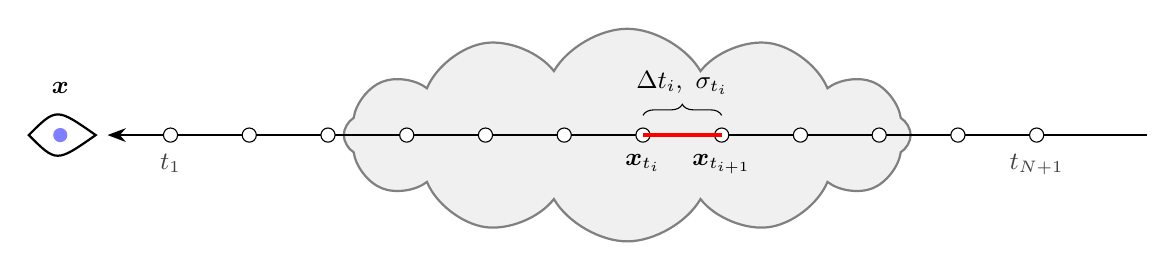
\begin{tikzpicture}[every node/.style={font=\small}]
% eye
\draw[thick] (0,0) .. controls (0.35,0.35) .. (0.85,0) .. controls (0.35,-0.35) .. cycle;
\fill[blue!50] (0.4,0) circle (0.09);
\node[above] at (0.4,0.4) {$\boldsymbol{x}$};
% cloud
\node[cloud,cloud puffs=12,cloud puff arc=120,aspect=2.4,draw=gray,thick,fill=gray!12,minimum width=7.2cm,minimum height=2.7cm] at (7.6,0) {};
% ray
\draw[thick,-{Stealth}] (14.2,0) -- (1.0,0);
\foreach \i in {0,...,11} {\draw[fill=white] (1.8+1.0*\i,0) circle (0.09);}
\draw[red,very thick] (7.8,0)--(8.8,0);
\node[below] at (7.8,-0.12) {$\boldsymbol{x}_{t_i}$};
\node[below] at (8.8,-0.12) {$\boldsymbol{x}_{t_{i+1}}$};
\draw[decorate,decoration={brace,amplitude=4pt}] (7.8,0.25)--(8.8,0.25) node[midway,above=4pt]{$\Delta t_i,\ \sigma_{t_i}$};
\node[below,gray!50!black] at (1.8,-0.12) {$t_1$};
\node[below,gray!50!black] at (12.8,-0.12) {$t_{N+1}$};
\end{tikzpicture}
\caption{Ray marching through an emitting/absorbing medium (redrawn from slides 3--6; original ray-marching figures by I.\ Gkioulekas). Within each segment the density $\sigma_{t_i}$ and the emission $\Le(\xx_{t_i},\om)$ are assumed constant.}
\end{figure}

\paragraph{Medium model.} The medium is \emph{absorbing and emitting}: every infinitesimal piece of volume emits light (colour) and absorbs part of the light passing through it. Absorption is governed by the density $\sigma$ and the \emph{transmittance}.

\begin{definition}[Transmittance]
For two points $\xx_a=\xx_{t_a}$ and $\xx_b=\xx_{t_b}$ on a ray, with $t_a<t_b$, the transmittance is the fraction of light that survives the trip between them,
\[
T(\xx_a,\xx_b)=\exp\!\Big(-\!\int_{t_a}^{t_b}\sigma(\xx_s)\dif s\Big)\in(0,1].
\]
\end{definition}

\begin{lemma}[A homogeneous emitting segment]\label{lem:segment}
Consider a segment of length $\Delta t$ with constant density $\sigma$ and constant emission $\Le$. The radiance it delivers to its near end, ignoring everything outside the segment, is
\[
\int_0^{\Delta t} e^{-\sigma s}\,\sigma\,\Le\dif s=\big(1-e^{-\sigma\Delta t}\big)\Le .
\]
\end{lemma}
\begin{proof}
Light emitted at depth $s$ inside the segment is attenuated by $e^{-\sigma s}$ before leaving it, and the amount emitted per unit length is $\sigma\Le$. Hence $\int_0^{\Delta t}\sigma\Le e^{-\sigma s}\dif s=\Le\,[-e^{-\sigma s}]_0^{\Delta t}=\Le(1-e^{-\sigma\Delta t})$.
\end{proof}

\begin{intuition}
The factor $\alpha=1-e^{-\sigma\Delta t}$ is the segment's \emph{opacity}: the probability that the ray is ``stopped'' (and thus sees the emitted colour) inside it. Thin or dilute segments ($\sigma\Delta t\ll1$) have $\alpha\approx\sigma\Delta t$; a thick one ($\sigma\Delta t\gg1$) has $\alpha\to1$ and is a solid wall. Example: $\sigma\Delta t=0.5\Rightarrow\alpha=0.39$, and $\sigma\Delta t=3\Rightarrow\alpha=0.95$.
\end{intuition}

\subsection{Transmittance as a recursion \sref{4--6}}

The light emitted by segment $i$ must still travel through all the segments between it and the camera; this is where $T(\xx,\xx_{t_i})$ enters (slide~4).

\begin{lemma}[Multiplicativity of transmittance]\label{lem:mult}
With $T_i\equiv T(\xx,\xx_{t_i})$ we have the base case $T_1=1$ and the recursion
\[
T_i=T_{i-1}\,e^{-\sigma_{t_{i-1}}\Delta t_{i-1}}\quad(i\ge2),\qquad\text{hence}\qquad T_i=\exp\!\Big(-\sum_{j<i}\sigma_{t_j}\Delta t_j\Big).
\]
(Slide~4 writes $\Delta t$; slide~6 shows that it may depend on $i$.)
\end{lemma}
\begin{proof}
$T_1=1$ because no medium lies between the camera and the first sample. For $i\ge2$, split the integral in $T$ at $t_{i-1}$: $\int_{t_1}^{t_i}\sigma=\int_{t_1}^{t_{i-1}}\sigma+\int_{t_{i-1}}^{t_i}\sigma$, and the exponential of a sum is a product. On the last segment $\sigma$ is constant, so the second integral equals $\sigma_{t_{i-1}}\Delta t_{i-1}$. Unrolling the recursion gives the closed form.
\end{proof}

\begin{theorem}[Discrete volume rendering]\label{thm:render}
For a ray with segments as above, the radiance reaching the camera is
\[
L(\xx,\om)=\sum_{i=1}^{N}T(\xx,\xx_{t_i})\,\big(1-e^{-\sigma_{t_i}\Delta t_i}\big)\,\Le(\xx_{t_i},\om)
=\sum_{i=1}^{N}w_i\,\cc_i,
\]
where $w_i=T_i\alpha_i$, $\alpha_i=1-e^{-\sigma_{t_i}\Delta t_i}$ and $\cc_i=\Le(\xx_{t_i},\om)$.
\end{theorem}
\begin{proof}
By Lemma~\ref{lem:segment} segment $i$ emits $\alpha_i\cc_i$ at its own near end; by Lemma~\ref{lem:mult} a fraction $T_i$ of it survives the way to the camera. Light emission is additive, so we sum over segments.
\end{proof}

\begin{intuition}
Standing at the camera you walk along the ray. At every segment you ask two questions: ``did the light from here survive everything in front of me?'' ($T_i$) and ``does this segment actually emit anything?'' ($\alpha_i\cc_i$). The weight $w_i$ is ``how much segment $i$ contributes to the pixel''; this is the quantity that colours the segments red/yellow on slides~32--33 and that will drive hierarchical sampling (Section~7).
\end{intuition}

\begin{algorithm}[Ray marching, slide 5]\label{alg:march}
\begin{enumerate}[nosep]
\item Draw samples along the ray ($N$ segments, i.e.\ $N+1$ points); slide~5 uses uniform spacing.
\item Compute the transmittance $T_i$ between the camera and each sample (recursion of Lemma~\ref{lem:mult}).
\item Aggregate the contributions $T_i\alpha_i\cc_i$ over all segments to obtain the overall radiance (the pixel colour).
\end{enumerate}
\end{algorithm}

\begin{example}[Worked numbers]\label{ex:toy}
Take $N=4$ segments of length $\Delta t=0.5$, densities $\sigma=(0.2,\,2,\,3,\,0.4)$ and grey-level emissions $\Le=(0.2,\,0.9,\,0.5,\,0.3)$.
Then $\alpha=(0.095,\,0.632,\,0.777,\,0.181)$, $T=(1,\,0.905,\,0.333,\,0.074)$ and so $w=T\alpha=(0.095,\,0.572,\,0.259,\,0.014)$. The pixel value is
$0.095\cdot0.2+0.572\cdot0.9+0.259\cdot0.5+0.014\cdot0.3\approx0.667$.
Segment~2 dominates: it is dense \emph{and} close to the camera. Segment~4 is hidden: $T_4$ is only $0.074$ even though $\alpha_4=0.18$.
\end{example}

\begin{figure}[H]
\centering
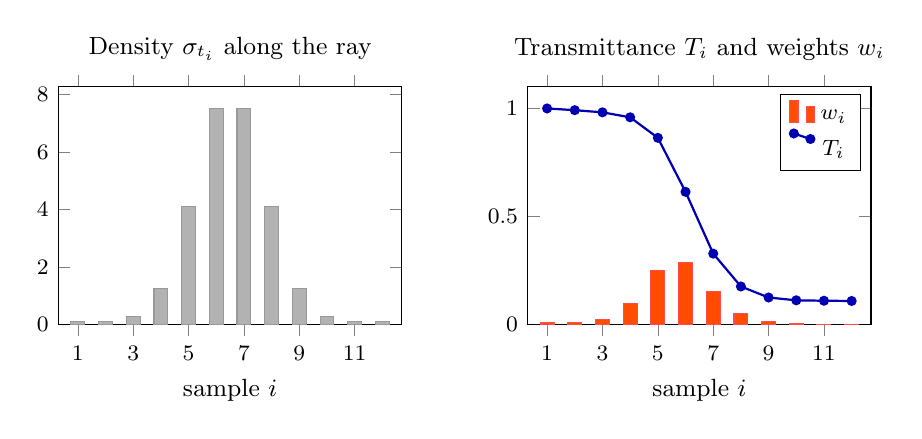
\begin{tikzpicture}
\begin{groupplot}[group style={group size=2 by 1,horizontal sep=1.6cm},
  width=0.49\linewidth,height=4.6cm,xmin=0.3,xmax=12.7,xtick={1,3,5,7,9,11},
  tick label style={font=\footnotesize},label style={font=\small},title style={font=\small}]
\nextgroupplot[title={Density $\sigma_{t_i}$ along the ray},xlabel={sample $i$},ybar,bar width=5pt,ymin=0,
  ]
\addplot[fill=gray!60,draw=gray!80] coordinates {(1,0.10)(2,0.12)(3,0.28)(4,1.26)(5,4.09)(6,7.51)(7,7.51)(8,4.09)(9,1.26)(10,0.28)(11,0.12)(12,0.10)};
\nextgroupplot[title={Transmittance $T_i$ and weights $w_i$},xlabel={sample $i$},ybar,bar width=5pt,ymin=0,ymax=1.1,
  legend style={font=\footnotesize,at={(0.97,0.97)},anchor=north east}]
\addplot[fill=red!70!yellow,draw=red!70] coordinates {(1,0.008)(2,0.009)(3,0.023)(4,0.096)(5,0.250)(6,0.285)(7,0.153)(8,0.051)(9,0.012)(10,0.003)(11,0.001)(12,0.001)};
\addplot[blue!70!black,thick,mark=*,mark size=1.4pt,sharp plot] coordinates {(1,1.000)(2,0.992)(3,0.982)(4,0.959)(5,0.864)(6,0.614)(7,0.328)(8,0.176)(9,0.125)(10,0.112)(11,0.110)(12,0.109)};
\legend{$w_i$,$T_i$}
\end{groupplot}
\end{tikzpicture}
\caption{Original illustration (not in the slides): a ray with 12 segments of length $1/12$ crossing a dense blob centred at the middle of the ray ($\sigma_{t_i}=0.1+8e^{-((t_i-0.5)/0.15)^2}$ at segment midpoints). Transmittance drops while the ray crosses the blob and the weights $w_i$ peak at the near side of the blob --- the first dense samples hide the ones behind. $\sum_iw_i=0.89$ and $T_{N+1}=0.11$.}
\end{figure}

\subsection{Enabling background radiance \sref{7}}

If the ray does not end inside the medium but hits an opaque surface or a background (the grey wall $\xx_z$ on slide~7), the light that survives the whole medium adds one more term:
\[
L(\xx,\om)=\sum_{i=1}^{N}T(\xx,\xx_{t_i})\big(1-e^{-\sigma_{t_i}\Delta t}\big)\Le(\xx_{t_i},\om)\;+\;T(\xx,\xx_{t_{N+1}})\,L(\xx_z,\om).
\]

\begin{proposition}[Weights sum to one]\label{prop:sum1}
With $w_i=T_i\alpha_i$ we have $w_i=T_i-T_{i+1}$ and therefore
\[
\sum_{i=1}^{N}w_i+T_{N+1}=1 .
\]
Consequently the rendered colour is a \emph{convex combination} of the segment colours and the background colour, and $T_{N+1}=1-\sum_iw_i$ is the \emph{background mask}.
\end{proposition}
\begin{proof}
By Lemma~\ref{lem:mult}, $T_{i+1}=T_ie^{-\sigma_{t_i}\Delta t_i}=T_i(1-\alpha_i)$, so $T_i-T_{i+1}=T_i\alpha_i=w_i$. The sum telescopes: $\sum_{i=1}^Nw_i=T_1-T_{N+1}=1-T_{N+1}$.
\end{proof}

\begin{intuition}
This is \emph{alpha compositing}. Every segment ``paints'' with opacity $\alpha_i$ over what is behind it; whatever the medium lets through ($T_{N+1}$) shows the background. Numerically, in Example~\ref{ex:toy} the weights sum to $0.939$ and $T_5=0.061$; with a white background ($L=1$) the pixel becomes $0.667+0.061\cdot 1=0.728$. For synthetic scenes with a white background one therefore renders $\hat C=\sum_iw_i\cc_i+(1-\sum_iw_i)\cdot 1$. In the same way, $T_{N+1}$ is a soft ``this ray hits nothing'' mask.
\end{intuition}

\subsection{Summary: computational volume rendering \sref{8}}

If we can compute (a)~a per-point density $\sigma_{t_i}\equiv\sigma(\xx_{t_i})$ and (b)~a per-point, per-direction emitted light $\Le(\xx_{t_i},\om)$, then we can render \emph{any} ray through the medium, hence an image from any camera viewpoint using $H\times W$ rays (one per pixel).

\begin{proposition}[Differentiability of the renderer]\label{prop:grad}
Let $\hat C=\sum_iw_i\cc_i+T_{N+1}L_{\rm bg}$. Then
\[
\frac{\partial\hat C}{\partial\cc_i}=w_i,\qquad
\frac{\partial\hat C}{\partial\sigma_{t_k}}=\Delta t_k\Big(T_{k+1}\,\cc_k-\sum_{i>k}w_i\cc_i-T_{N+1}L_{\rm bg}\Big).
\]
\end{proposition}
\begin{proof}
The first identity is immediate. For $\sigma_{t_k}$: $\alpha_k$ depends on it with $\partial\alpha_k/\partial\sigma_{t_k}=\Delta t_ke^{-\sigma_{t_k}\Delta t_k}$, so the term $w_k\cc_k$ contributes $T_k\Delta t_ke^{-\sigma_{t_k}\Delta t_k}\cc_k=\Delta t_kT_{k+1}\cc_k$. Moreover $T_i$ for every $i>k$ (and $T_{N+1}$) contains $e^{-\sigma_{t_k}\Delta t_k}$, so $\partial T_i/\partial\sigma_{t_k}=-\Delta t_kT_i$ and $w_i=T_i\alpha_i$ gives $-\Delta t_kw_i\cc_i$; likewise for the background term.
\end{proof}

\begin{intuition}
Increasing the density at sample $k$ has two opposite effects (slide~8's red note: the pipeline is differentiable). It makes sample $k$'s own colour more visible (positive term) but it also hides everything behind it (negative terms). Gradient descent on a photometric loss thus ``pushes density'' to where it explains the pixel and removes it where it would wrongly occlude. The same holds for the camera parameters whenever density and emission are differentiable functions of position and direction.
\end{intuition}

%==============================================================
\section{Volumes: Rendering and Representation \sref{9--10}}
%==============================================================

Slides~9--10 split the problem into two boxes:
\[
\underbrace{\begin{matrix}\sigma_{t_i}\equiv\sigma(\xx_{t_i})\\ \Le(\xx_{t_i},\om)\end{matrix}}_{\text{representation: ``How to represent volumes?''}}
\;\longrightarrow\;
\underbrace{L(\xx,\om)}_{\text{rendering algorithm (done)}}
\]
The rendering algorithm is fixed; what remains is a \emph{representation} from which the density and the emitted light can be computed pointwise.

\slideimg{9}{4.2cm}{A volumetric example (smoke-like plume): volumes can be rich and view-dependent, and we need a representation that can encode them. Figure credits as on the slide.}

\begin{figure}[H]
\centering
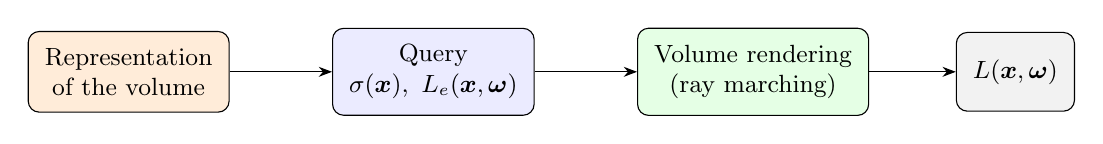
\begin{tikzpicture}[every node/.style={font=\small},box/.style={draw,rounded corners,minimum height=1cm,align=center,inner sep=6pt}]
\node[box,fill=orange!15] (rep) {Representation\\ of the volume};
\node[box,fill=blue!8,right=1.3cm of rep] (q) {Query\\ $\sigma(\xx),\ \Le(\xx,\om)$};
\node[box,fill=green!10,right=1.3cm of q] (r) {Volume rendering\\ (ray marching)};
\node[box,fill=gray!10,right=1.1cm of r] (o) {$L(\xx,\om)$};
\draw[-{Stealth}] (rep)--(q); \draw[-{Stealth}] (q)--(r); \draw[-{Stealth}] (r)--(o);
\end{tikzpicture}
\caption{Division of labour in slides~9--10: the representation only has to answer pointwise queries; ray marching does the rest.}
\end{figure}

\subsection{Option 1: a grid --- Grid Representation \sref{11--17}}

\begin{definition}[Voxel-grid volume]
A grid stores a positive scalar in each voxel, $\sigma[x,y,z]\in\R^+$ (the density), and --- for emission --- a colour $\cc[x,y,z]\in[0,1]^3$. Since the lookup of an arbitrary real-valued point $\xx$ is not a voxel index, slide~11 asks: \emph{how to obtain $\sigma(\xx)$ for arbitrary $\xx$?} The answer is interpolation.
\end{definition}

\subsubsection*{Trilinear interpolation \sref{12}}

Let $\xx$ fall into a cell whose eight corners carry the values $\sigma_{ijk}$, $i,j,k\in\{0,1\}$. Let $(u,v,w)\in[0,1]^3$ be the local coordinates of $\xx$ in the cell, and set $u_1=u,\ u_0=1-u$ (same for $v,w$).

\begin{definition}[Trilinear interpolation]
$\displaystyle \sigma(\xx)=\sum_{i,j,k\in\{0,1\}}u_i\,v_j\,w_k\,\sigma_{ijk}.$
It is the 3D equivalent of bilinear interpolation.
\end{definition}

\begin{lemma}[Properties of trilinear interpolation]\label{lem:trilin}
(i)~The weights $\lambda_{ijk}=u_iv_jw_k$ are non-negative and sum to $1$.
(ii)~The weight of a corner equals the volume of the box spanned by $\xx$ and the \emph{opposite} corner.
(iii)~$\sigma$ is linear in each of $u,v,w$ separately, reproduces the corner values, and is continuous across cell boundaries.
(iv)~$\partial\sigma(\xx)/\partial\sigma_{ijk}=\lambda_{ijk}$: the interpolation is differentiable w.r.t.\ the stored corner values.
\end{lemma}
\begin{proof}
(i)~$\sum\lambda_{ijk}=(u_0+u_1)(v_0+v_1)(w_0+w_1)=1$. (ii)~The box between $\xx$ and the corner $(0,0,0)$ has side lengths $u,v,w$, so its volume is $uvw=\lambda_{111}$; the other corners follow by symmetry (e.g.\ $\lambda_{000}=(1-u)(1-v)(1-w)$ is the box towards $(1,1,1)$). (iii)~Fix $v,w$: $\sigma$ is a convex combination $(1-u)a+ub$, linear in $u$; at a corner one $\lambda$ equals $1$ and the others vanish. On a shared face, say $u=1$, the formula only involves the four corners of that face, so neighbouring cells agree. (iv)~Linearity in the $\sigma_{ijk}$.
\end{proof}

\begin{figure}[H]
\centering
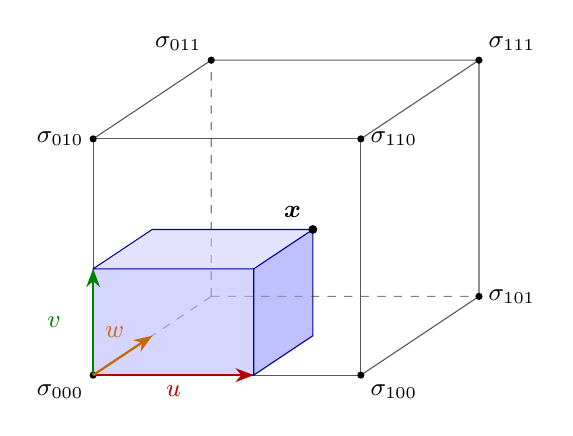
\begin{tikzpicture}[x={(3.4cm,0cm)},y={(0cm,3.0cm)},z={(1.5cm,1.0cm)},every node/.style={font=\small}]
\def\u{0.6}\def\v{0.45}\def\w{0.5}
% hidden edges
\draw[gray,dashed] (0,0,1)--(1,0,1) (0,0,1)--(0,1,1) (0,0,1)--(0,0,0);
% visible cube edges
\draw[gray!70!black] (0,0,0)--(1,0,0)--(1,1,0)--(0,1,0)--cycle;
\draw[gray!70!black] (0,1,0)--(0,1,1)--(1,1,1)--(1,1,0);
\draw[gray!70!black] (1,0,0)--(1,0,1)--(1,1,1);
% opposite sub-box (volume = weight of corner 111)
\fill[blue!30,opacity=0.55] (0,0,0)--(\u,0,0)--(\u,\v,0)--(0,\v,0)--cycle;
\fill[blue!45,opacity=0.55] (\u,0,0)--(\u,0,\w)--(\u,\v,\w)--(\u,\v,0)--cycle;
\fill[blue!20,opacity=0.55] (0,\v,0)--(\u,\v,0)--(\u,\v,\w)--(0,\v,\w)--cycle;
\draw[blue!60!black] (0,0,0)--(\u,0,0)--(\u,\v,0)--(0,\v,0)--cycle (\u,0,0)--(\u,0,\w)--(\u,\v,\w)--(\u,\v,0) (0,\v,0)--(0,\v,\w)--(\u,\v,\w);
\fill (\u,\v,\w) circle (1.6pt) node[above left=1pt]{$\boldsymbol{x}$};
% corners
\foreach \p/\l/\a in {{0,0,0}/{\sigma_{000}}/below left,{1,0,0}/{\sigma_{100}}/below right,{0,1,0}/{\sigma_{010}}/left,{1,1,0}/{\sigma_{110}}/right,{1,0,1}/{\sigma_{101}}/right,{1,1,1}/{\sigma_{111}}/above right,{0,1,1}/{\sigma_{011}}/above left}
  {\fill (\p) circle(1.3pt) node[\a]{$\l$};}
% axes
\draw[-{Stealth},red!70!black,thick] (0,0,0)--(\u,0,0) node[pos=0.5,below]{$u$};
\draw[-{Stealth},green!50!black,thick] (0,0,0)--(0,\v,0) node[pos=0.5,left=8pt]{$v$};
\draw[-{Stealth},orange!80!black,thick] (0,0,0)--(0,0,0.5) node[pos=0.7,above left]{$w$};
\end{tikzpicture}
\caption{Trilinear interpolation (redrawn from slide 12). The shaded box between $\boldsymbol x$ and corner $(0,0,0)$ has volume $uvw$ and is the weight of the \emph{opposite} corner $\sigma_{111}$; the other seven weights are the volumes of the other seven sub-boxes, which tile the cell.}
\end{figure}

\begin{intuition}
Imagine standing in the cell and drawing the three planes through yourself parallel to the faces: they cut the cell into eight little boxes. Each corner is weighted by the box \emph{on the other side} of you --- the closer you are to a corner, the bigger the opposite box, hence the larger its weight. In 1D this is just $(1-u)a+ub$; e.g.\ for $u=0.25$ the nearer value gets weight $0.75$. In 3D with $(u,v,w)=(0.6,0.45,0.5)$ as in the figure, $\lambda_{111}=0.6\cdot0.45\cdot0.5=0.135$ and $\lambda_{000}=0.4\cdot0.55\cdot0.5=0.11$.
\end{intuition}

\subsubsection*{Emission on the grid \sref{13--15}}

\emph{Q: how do we model view-dependent emission $\Le(\xx,\om)$?} The grid answer (slide~13) is to \emph{ignore} view dependence: $\Le(\xx,\om)\equiv\cc(\xx)$. Slide~14 therefore stores a colour $\cc[x,y,z]\in[0,1]^3$ next to the density in every voxel, and trilinear interpolation is applied to both.

\slideimg{14, 15}{4.4cm}{Left: a chair stored as a coloured voxel grid (slide 14). Right: an emission-only rendering of a cloud and the corresponding density voxel grid, downsampled for visualization (slide 15).}

\slideimg{16}{4.2cm}{Voxel grids are everywhere in medical imaging: a 3D brain volume with voxel $(i,j,k)$ and a 2D MRI slice with pixel $(i,j)$. Figure credits: www.hindawi.com/journals/cmmm/2015/450341.}

\subsubsection*{Limits of the grid \sref{17}}

\slideimg{17}{4.2cm}{Slide 17: a real captured scene (red car) --- grids ``cannot model view-dependent effects'' such as the car's reflections, and their size grows cubically with the scene dimension. Video credits: Mildenhall et al., ECCV 2020 (NeRF).}

\begin{proposition}[Cubic memory growth]\label{prop:cubic}
A dense grid with resolution $N$ per axis and $b$ bytes per voxel needs $N^3b$ bytes. Doubling the resolution multiplies memory (and training/rendering cost per volume) by $8$.
\end{proposition}
\begin{intuition}
With $\sigma$ and an RGB colour in 32-bit floats ($b=16$ bytes), $N=128$ costs $33.6$~MB, $N=512$ already $2.1$~GB, and $N=1024$ about $17.2$~GB --- for a scene that is mostly empty space. Together with the lack of view-dependent colour this is what motivates the MLP of the next section, and later sparse (Plenoxels) and hash-based (Instant-NGP) hybrids.
\end{intuition}

%==============================================================
\section{Neural Radiance Fields \sref{18--20}}
%==============================================================

\emph{Volumes: Rendering and Representation, Option 2: An MLP} (slide~18). Instead of storing values on a lattice, store them in the weights of a neural network.

\begin{definition}[Neural Radiance Field]\label{def:nerf}
A NeRF is a multilayer perceptron (MLP)
\[
f_\theta:\ (\xx,\om)\longmapsto(\sigma,\cc),\qquad \sigma\in\R^+,\quad\cc\in[0,1]^3 ,
\]
such that (1)~given an input point it predicts the density, and (2)~given a point \emph{and} a viewing direction it predicts the radiance (colour). The scene is represented \emph{entirely} by the weights $\theta$.
\end{definition}

\begin{proposition}[Density is view-independent by design]\label{prop:viewindep}
If $\om$ is injected only after the layer that produces $\sigma$, then $\sigma=\sigma(\xx)$ does not depend on $\om$, while $\cc=\cc(\xx,\om)$ may.
\end{proposition}
\begin{proof}
$\sigma$ is computed by a function composition that has $\xx$ (or features of it) as its only input; $\om$ is concatenated afterwards, so no path from $\om$ to $\sigma$ exists in the computation graph.
\end{proof}

\begin{intuition}
Physically, whether there is matter at a point cannot depend on where you look from, whereas the colour of a shiny surface can. Slide~18 asks us to ensure this ``with designing the MLP that density only depends on $\xx$''; this is what the architecture of Figure~\ref{fig:arch} does. This is a built-in inductive bias which makes the 3D structure consistent across views.
\end{intuition}

\begin{figure}[H]
\centering
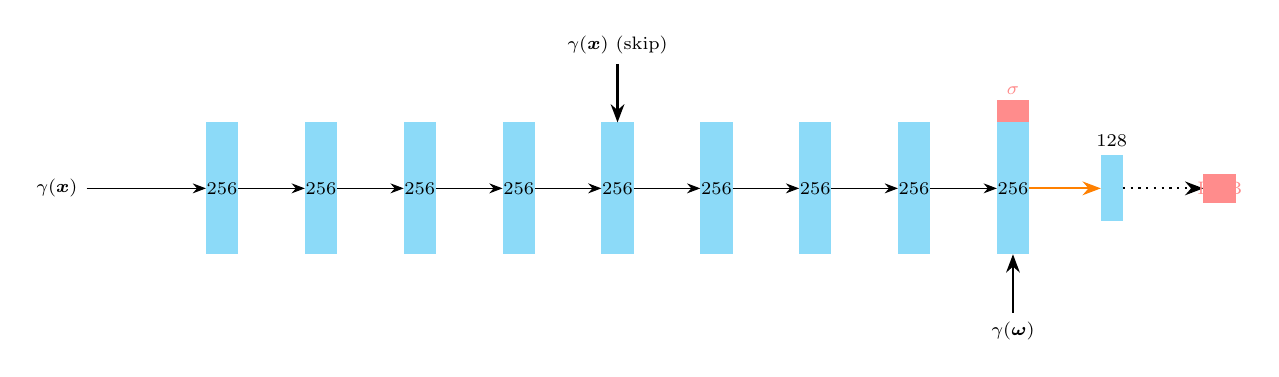
\begin{tikzpicture}[every node/.style={font=\scriptsize},scale=0.93,transform shape]
\foreach \i in {1,...,9} {
  \fill[cyan!45] (1.35*\i-0.22,-0.9) rectangle (1.35*\i+0.22,0.9);
  \node at (1.35*\i,0) {256};}
\foreach \i in {1,...,8} {\pgfmathtruncatemacro{\j}{\i+1}\draw[-{Stealth}] (1.35*\i+0.22,0)--(1.35*\j-0.22,0);}
\draw[-{Stealth}] (-0.5,0)--(1.35-0.22,0) node[pos=0,left]{$\gamma(\boldsymbol x)$};
\draw[-{Stealth},thick] (1.35*5,1.7)--(1.35*5,0.9) node[pos=0,above]{$\gamma(\boldsymbol x)$ (skip)};
% sigma
\fill[red!45] (1.35*9-0.22,0.9) rectangle (1.35*9+0.22,1.2) node[midway,above=3pt]{$\sigma$};
% direction
\draw[-{Stealth},thick] (1.35*9,-1.7)--(1.35*9,-0.9) node[pos=0,below]{$\gamma(\boldsymbol\omega)$};
\draw[orange,-{Stealth},thick] (1.35*9+0.22,0)--(1.35*10-0.15,0);
\fill[cyan!45] (1.35*10-0.15,-0.45) rectangle (1.35*10+0.15,0.45);
\node[above] at (1.35*10,0.45) {128};
\draw[dotted,-{Stealth},thick] (1.35*10+0.15,0)--(1.35*11-0.1,0);
\fill[red!45] (1.35*11-0.1,-0.2) rectangle (1.35*11+0.35,0.2) node[midway]{RGB};
\end{tikzpicture}
\caption{The NeRF MLP (redrawn from slides 18 and 24): fully connected blocks of width 256; the encoded position is fed again at the fifth block (skip connection); the density $\sigma$ is read out \emph{before} the viewing direction is concatenated; one extra 128-unit layer sees $\gamma(\om)$ and outputs the RGB colour. Typical choices: ReLU hidden units, a non-negative activation (ReLU/softplus) for $\sigma$, sigmoid for RGB, so that $\sigma\in\R^+$ and $\cc\in[0,1]^3$.}\label{fig:arch}
\end{figure}

\textbf{How to train this MLP?} (slide~20). Key idea: \emph{learn a 3D representation consistent with the observed views.} The next section turns this sentence into a loss.

%==============================================================
\section{Learning Neural Radiance Fields \sref{21--24}}
%==============================================================

\subsection{From pixels to rays \sref{21--22}}

\begin{definition}[Camera ray]
Given a pixel $\boldsymbol p=(u,v)$ and camera parameters $\pi=(K,R,\boldsymbol t_c)$ (intrinsics $K$, world-from-camera rotation $R$ and camera centre $\boldsymbol t_c$), the ray through $\boldsymbol p$ is
\[
\xx_t=\boldsymbol o+t\,\dd,\qquad \boldsymbol o=\boldsymbol t_c,\quad \dd=\frac{RK^{-1}(u,v,1)^\top}{\|RK^{-1}(u,v,1)^\top\|},\quad t\ge0 .
\]
The slides abbreviate this as the map (pixel, camera) $\to$ ray, and the viewing direction fed to the network is $\om=-\dd$ (or $\dd$, by convention).
\end{definition}

\begin{definition}[View-synthesis loss]
Let $\mathrm{render}(\boldsymbol p,\pi;f_\theta)$ be the volume-rendered colour (Theorem~\ref{thm:render}) of the ray through pixel $\boldsymbol p$ of the camera $\pi$ when the volume is given by $f_\theta$. The NeRF is trained by
\[
\min_\theta\ \sum_{I}\sum_{\boldsymbol p}\big\|\mathrm{render}(\boldsymbol p,\pi;f_\theta)-I[\boldsymbol p]\big\|^2 ,
\]
where $I$ runs over the training images and $\boldsymbol p$ over their pixels.
\end{definition}

\begin{figure}[H]
\centering
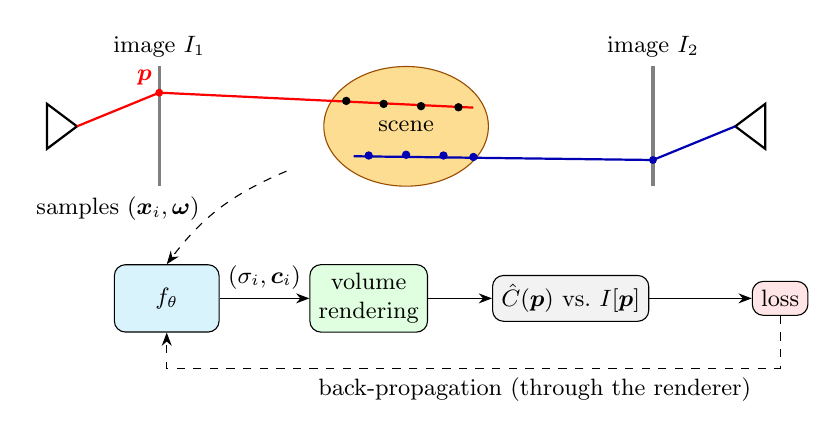
\begin{tikzpicture}[every node/.style={font=\small},scale=0.95,transform shape]
% scene
\fill[yellow!40!orange!40,draw=orange!60!black] (0,1.7) ellipse (1.1cm and 0.8cm);
\node at (0,1.7) {scene};
% camera A
\draw[thick] (-4.4,1.7)--(-4.8,2.0)--(-4.8,1.4)--cycle;
\draw[very thick,gray] (-3.3,0.9)--(-3.3,2.5);
\node[above] at (-3.3,2.5) {image $I_1$};
\draw[red,thick] (-4.4,1.7)--(-3.3,2.15)--(0.9,1.95);
\fill[red] (-3.3,2.15) circle(1.5pt) node[above left=-1pt]{$\boldsymbol p$};
\foreach \x/\y in {-0.8/2.04,-0.3/2.0,0.2/1.97,0.7/1.955} {\fill (\x,\y) circle(1.6pt);}
% camera B
\draw[thick] (4.4,1.7)--(4.8,2.0)--(4.8,1.4)--cycle;
\draw[very thick,gray] (3.3,0.9)--(3.3,2.5);
\node[above] at (3.3,2.5) {image $I_2$};
\draw[blue!70!black,thick] (4.4,1.7)--(3.3,1.25)--(-0.7,1.3);
\fill[blue!70!black] (3.3,1.25) circle(1.5pt);
\foreach \x/\y in {-0.5/1.31,0.0/1.32,0.5/1.31,0.9/1.29} {\fill[blue!70!black] (\x,\y) circle(1.6pt);}
% pipeline
\node[draw,rounded corners,fill=cyan!15,minimum width=1.4cm,minimum height=0.9cm] (f) at (-3.2,-0.6) {$f_\theta$};
\node[draw,rounded corners,fill=green!12,align=center] (vr) at (-0.5,-0.6) {volume\\ rendering};
\node[draw,rounded corners,fill=gray!10,align=center] (ch) at (2.2,-0.6) {$\hat C(\boldsymbol p)$ vs.\ $I[\boldsymbol p]$};
\node[draw,rounded corners,fill=red!10] (ls) at (5.0,-0.6) {loss};
\draw[-{Stealth}] (f)--(vr) node[midway,above]{$(\sigma_i,\boldsymbol c_i)$};
\draw[-{Stealth}] (vr)--(ch); \draw[-{Stealth}] (ch)--(ls);
\draw[-{Stealth},dashed] (-1.6,1.1) to[bend right=15] node[midway,left,xshift=-4pt]{samples $(\xx_i,\om)$} (f.north);
\draw[-{Stealth},dashed] (ls.south) -- ++(0,-0.7) -| node[pos=0.2,below]{back-propagation (through the renderer)} (f.south);
\end{tikzpicture}
\caption{Learning a NeRF (redrawn and simplified from slides 21--22). Rays from two cameras are marched; the 3D points are sent to $f_\theta$, whose outputs are composited by volume rendering and compared with the observed pixel. The gradient flows back through the (differentiable) renderer to $\theta$.}
\end{figure}

\begin{intuition}
The loss never mentions 3D. It only says: ``if I shoot the ray of pixel $\boldsymbol p$ through my current cloud, I should get the pixel's colour.'' But a 3D point on the visible surface lies on the rays of many cameras, and the only way to be right for \emph{all} of them simultaneously is to put density at the correct place with a colour that is consistent across views. This is why slide~23 requires typically more than 50 images with \emph{known} camera parameters (in practice obtained with structure-from-motion).
\end{intuition}

\subsection{Mini-batches of rays \sref{23}}

A single image already has $H\times W$ rays (e.g.\ $800\times800=640{,}000$) and each ray needs many network queries (Section~7), so we cannot back-propagate through all of them. ``In practice, randomly sample a few pixels (rays) per optimisation iteration.''

\begin{proposition}[Unbiased stochastic gradients]
Let $\mathcal L(\theta)=\frac1{|\mathcal P|}\sum_{(I,\boldsymbol p)\in\mathcal P}\ell_{I,\boldsymbol p}(\theta)$ be the average per-ray loss over all training pixels $\mathcal P$, and $B$ a batch of $m$ pixels drawn uniformly (with replacement). Then $\E_B\big[\frac1m\sum_{b\in B}\nabla\ell_b\big]=\nabla\mathcal L(\theta)$.
\end{proposition}
\begin{proof}
Each draw is uniform, so $\E[\nabla\ell_b]=\frac1{|\mathcal P|}\sum_{p\in\mathcal P}\nabla\ell_p=\nabla\mathcal L$; the average of $m$ such expectations is the same.
\end{proof}
\begin{intuition}
It is the usual stochastic gradient descent, except that the ``training examples'' are individual rays, not whole images. Random rays from random images also decorrelate the updates, much like random mini-batches.
\end{intuition}

\begin{algorithm}[NeRF training loop, slide 24]\label{alg:train}
\begin{enumerate}[nosep]
\item \textbf{Acquire} multiple images of a scene with associated camera viewpoints.
\item \textbf{Design} a neural network $(\sigma,\cc)=f_\theta(\xx,\om)$.
\item \textbf{Train} with a view-synthesis loss using volume rendering: repeat \emph{(a)} draw a batch of (image, pixel) pairs; \emph{(b)} build their rays; \emph{(c)} sample points along each ray; \emph{(d)} query $f_\theta$; \emph{(e)} composite with Theorem~\ref{thm:render}; \emph{(f)} compute the squared error to the pixel colours; \emph{(g)} update $\theta$ by gradient descent.
\end{enumerate}
\end{algorithm}

\slideimg{24}{4.2cm}{Step 1 of the recipe: many camera viewpoints around the object (here a drum set); each camera is paired with its image. Figure credits: Mildenhall et al., ECCV 2020 (NeRF).}

%==============================================================
\section{Learning Neural Radiance Fields: An Initial Attempt \sref{25}}
%==============================================================

Feeding the raw coordinates $(\xx,\om)$ to the MLP and training as above gives disappointing results (slide~25): from 100 training images the network produces \emph{blurry} novel views --- \textbf{it cannot capture high-frequency details}.

\slideimg{25}{4.8cm}{Slide 25: 100 training images $\to$ optimised neural net $\to$ novel-view rendering of the lego scene (blurry result; first attempt without positional encoding). Figure credits: Mildenhall et al., ECCV 2020 (NeRF).}

%==============================================================
\section{Modeling High Frequencies: A Toy Problem \sref{26--30}}
%==============================================================

The slides isolate the phenomenon on a 2D toy problem: regress an image, $(x,y)\to f_\theta\to(r,g,b)$ (slide~26). A ``standard'' MLP returns a smooth, blurry image, because ReLU MLPs trained by gradient descent fit low frequencies first (\emph{spectral bias}). The remedy: lift the input to a vector of sines and cosines at geometrically increasing frequencies.

\slideimg{26, 27}{5cm}{Image regression toy problem: input image, result with a ``standard'' MLP (blurry), and result using positional encoding (sharp). Figure credits: Tancik et al., NeurIPS 2020 (Fourier Features).}

\begin{definition}[Positional encoding]\label{def:pe}
For a scalar or vector $\boldsymbol v$ (applied coordinate-wise) and a number of octaves $L$,
\[
\gamma(\boldsymbol v)=\big(\boldsymbol v,\ \sin(\boldsymbol v),\cos(\boldsymbol v),\ \sin(2\boldsymbol v),\cos(2\boldsymbol v),\ \sin(4\boldsymbol v),\cos(4\boldsymbol v),\dots,\ \sin(2^{L-1}\boldsymbol v),\cos(2^{L-1}\boldsymbol v)\big).
\]
(The slide lists the $\sin/\cos$ terms; the original NeRF also multiplies the argument by $\pi$, i.e.\ $\sin(2^k\pi v)$, for coordinates normalised to $[-1,1]$, and uses $L=10$ for positions and $L=4$ for directions. Whether $\boldsymbol v$ itself is kept is an implementation detail.) The network is now trained on $\gamma(\xx)$ and $\gamma(\om)$ instead of $\xx$ and $\om$.
\end{definition}

\begin{lemma}[$\gamma$ induces a shift-invariant similarity]\label{lem:gammakernel}
For scalars $v,v'$,
\[
\langle\gamma(v),\gamma(v')\rangle_{\sin/\cos}=\sum_{k=0}^{L-1}\cos\!\big(2^k(v-v')\big)
\]
which depends only on $v-v'$. For vectors, sum over the coordinates.
\end{lemma}
\begin{proof}
$\sin a\sin b+\cos a\cos b=\cos(a-b)$ applied with $a=2^kv$, $b=2^kv'$ for each $k$.
\end{proof}

\begin{figure}[H]
\centering
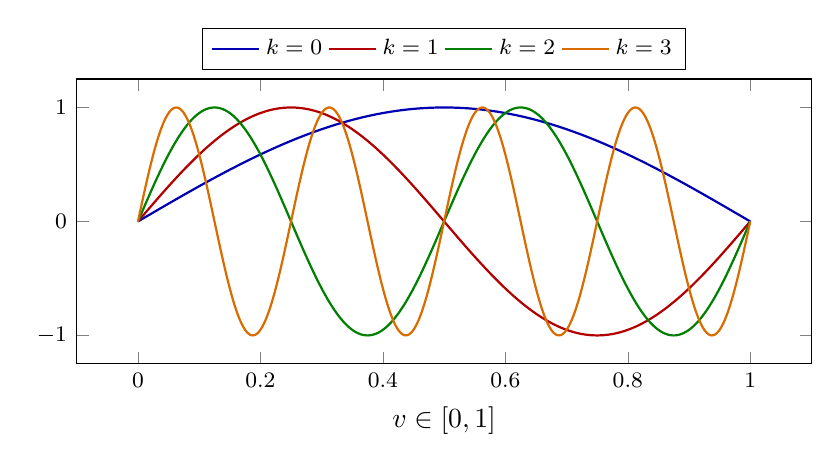
\begin{tikzpicture}
\begin{axis}[width=0.9\linewidth,height=5.2cm,xlabel={$v\in[0,1]$},ylabel={},domain=0:1,samples=400,
  ymin=-1.25,ymax=1.25,legend columns=4,legend style={font=\footnotesize,at={(0.5,1.03)},anchor=south},
  tick label style={font=\footnotesize},no markers]
\addplot[blue!70!black,thick]{sin(180*x)};
\addplot[red!70!black,thick]{sin(360*x)};
\addplot[green!50!black,thick]{sin(720*x)};
\addplot[orange!85!black,thick]{sin(1440*x)};
\legend{$k=0$,$k=1$,$k=2$,$k=3$}
\end{axis}
\end{tikzpicture}
\caption{Original illustration: the first four components $\sin(2^k\pi v)$ of the positional encoding. Each octave doubles the frequency, so a few components span a wide range of scales; with $L=10$ the finest component has a period of $2/2^{9}=1/256$ of the normalised coordinate range.}
\end{figure}

\begin{intuition}
Why does this help? Without encoding, two nearby points have nearly identical inputs, so the network treats them nearly identically (it is ``smooth'' in $\xx$). After encoding, the high-frequency components $\sin(2^{k}\cdot)$ with large $k$ change very fast with $\xx$: two points $0.004$ apart look completely different to the network, which can then give them different densities and colours. Lemma~\ref{lem:gammakernel} says the network's notion of ``similar points'' becomes a band-limited kernel with bandwidth $\approx 2^{L-1}$ that we can tune, rather than a very smooth one. This is the Fourier-features argument of Tancik et al.: ``Fourier features let networks learn high-frequency functions in low-dimensional domains''.
\end{intuition}

\slideimg{28}{4.8cm}{Slide 28: with positional encodings at the input, the same pipeline (100 training images $\to$ optimised neural net $\to$ novel views) produces a sharp lego bulldozer --- ``a great example that execution matters''. Figure credits: Mildenhall et al., ECCV 2020 (NeRF).}

\slideimg{29}{4.6cm}{Slide 29: NeRF (naive) vs.\ NeRF (with positional encoding) on the ``fern'' scene --- the encoded version recovers leaf detail. Figure credits: Mildenhall et al., ECCV 2020 (NeRF).}

\slideimg{30}{4.6cm}{Slide 30 (video frame): standard input vs.\ Fourier-feature input for a 3D shape, a 3D MRI and a 3D NeRF. Video credits: Tancik and Srinivasan et al., NeurIPS 2020 (Fourier Features Let Networks Learn High Frequency Functions in Low Dimensional Domains).}

%==============================================================
\section{Uniform to Hierarchical Sampling \sref{31--33}}
%==============================================================

The rendering sum of Theorem~\ref{thm:render} is a quadrature of the volume-rendering integral along the ray, and each term costs one MLP evaluation. Uniform spacing (slide~31) is wasteful: many samples fall in empty space or behind an opaque surface, where the weight $w_i$ is tiny. Slides~32--33 therefore reuse
\[
L(\xx,\om)=\sum_iw_i\,\cc_i,\qquad w_i=T_i\big(1-e^{-\sigma_{t_i}\Delta t}\big),
\]
where the \emph{weights indicate how much each segment contributes to the pixel value} (red = high, yellow = low). Strategy: (1)~sample points uniformly; (2)~sample \emph{more} points in the segments with large weights.

\begin{figure}[H]
\centering
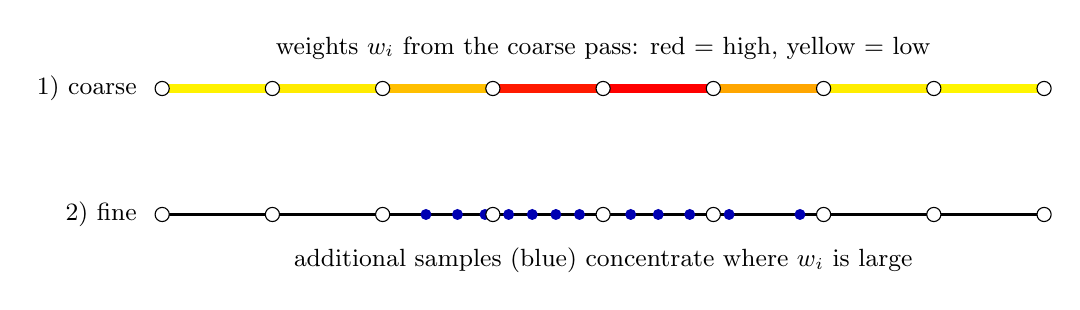
\begin{tikzpicture}[every node/.style={font=\small}]
\def\W{{0.05,0.08,0.25,0.9,1.0,0.35,0.07,0.04}}
% coarse pass
\node[left] at (-0.2,1.6) {1) coarse};
\draw[thick] (0,1.6)--(11.2,1.6);
\foreach \i in {0,...,7} {
  \pgfmathsetmacro{\wi}{\W[\i]}
  \pgfmathsetmacro{\pc}{100*\wi}
  \draw[line width=3.5pt,red!\pc!yellow] (1.4*\i+0.06,1.6)--(1.4*\i+1.34,1.6);}
\foreach \i in {0,...,8} {\draw[fill=white] (1.4*\i,1.6) circle(0.09);}
\node[above,align=center] at (5.6,1.85) {weights $w_i$ from the coarse pass: red = high, yellow = low};
% fine pass
\node[left] at (-0.2,0) {2) fine};
\draw[thick] (0,0)--(11.2,0);
\foreach \x in {0,1.4,2.8,11.2} {\draw[fill=white] (\x,0) circle(0.09);}
\foreach \x in {3.35,3.75,4.1,4.4,4.7,5.0,5.3,5.6,5.95,6.3,6.7,7.2,8.1} {\fill[blue!70!black] (\x,0) circle(0.07);}
\foreach \x in {4.2,5.6,7.0,8.4,9.8} {\draw[fill=white] (\x,0) circle(0.09);}
\node[below,align=center] at (5.6,-0.3) {additional samples (blue) concentrate where $w_i$ is large};
\end{tikzpicture}
\caption{Hierarchical sampling (redrawn and simplified from slides 31--33). A first, uniform ``coarse'' pass computes the weights; a second pass draws extra samples with density proportional to them. (Sample positions are schematic.)}
\end{figure}

\begin{definition}[Piecewise-constant PDF along the ray]
Normalise the coarse weights, $\hat w_i=w_i/\sum_jw_j$, and define the density on $[t_1,t_{N+1}]$ that equals $\hat w_i/\Delta t_i$ on the $i$-th segment and the cumulative distribution $F(t)=\int_{t_1}^tp(s)\dif s$, which is piecewise linear.
\end{definition}

\begin{lemma}[Inverse-transform sampling]\label{lem:invcdf}
If $U\sim\mathcal U[0,1]$ and $F$ is a strictly increasing CDF, then $t=F^{-1}(U)$ has CDF $F$.
\end{lemma}
\begin{proof}
$\Pr[F^{-1}(U)\le t]=\Pr[U\le F(t)]=F(t)$, since $F$ is monotonic and $U$ is uniform. (For a piecewise-linear CDF with flat parts, take the left-continuous generalised inverse.)
\end{proof}

\begin{algorithm}[Hierarchical sampling]\label{alg:hier}
\begin{enumerate}[nosep]
\item Sample $N_c$ points uniformly along the ray (one random point inside each of $N_c$ equal bins in the original NeRF) and evaluate the network (``coarse'' pass).
\item Compute the weights $w_i$ and the normalised piecewise-constant PDF $\hat w_i$.
\item Draw $N_f$ further points $t=F^{-1}(u_j)$ with $u_j\sim\mathcal U[0,1]$ (Lemma~\ref{lem:invcdf}).
\item Evaluate the network on the sorted union of all $N_c+N_f$ points and render the pixel (``fine'' pass). Original NeRF: $N_c=64$, $N_f=128$, with a coarse and a fine network, both supervised.
\end{enumerate}
\end{algorithm}

\begin{example}[Inverse CDF by hand]
Four bins of unit length on $t\in[0,4]$ with normalised weights $(0.1,0.5,0.3,0.1)$ give the CDF values $(0,0.1,0.6,0.9,1)$ at $t=0,1,2,3,4$. For $u=0.5$: $F(t)=0.5$ lies in bin~2 (between $0.1$ and $0.6$) at fraction $(0.5-0.1)/0.5=0.8$ of the way, so $t=1+0.8=1.8$. Half of the random numbers $u\in[0.1,0.6]$ fall in bin~2, so bin~2 receives half of the new samples although it is only a quarter of the ray length.
\end{example}

\begin{figure}[H]
\centering
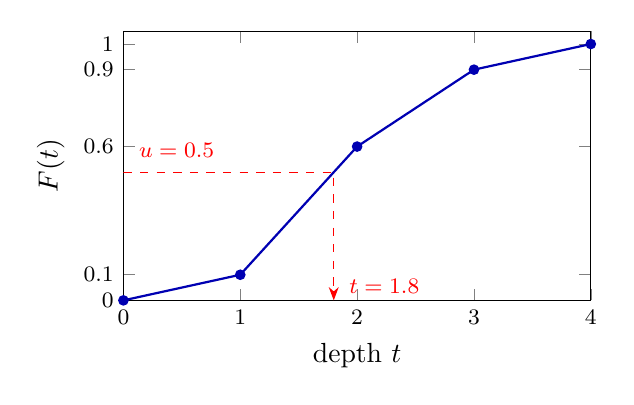
\begin{tikzpicture}
\begin{axis}[width=0.62\linewidth,height=5cm,xmin=0,xmax=4,ymin=0,ymax=1.05,xlabel={depth $t$},ylabel={$F(t)$},xtick={0,1,2,3,4},ytick={0,0.1,0.6,0.9,1},tick label style={font=\footnotesize}]
\addplot[blue!70!black,thick,mark=*,mark size=1.5pt] coordinates {(0,0)(1,0.1)(2,0.6)(3,0.9)(4,1)};
\draw[red,dashed,-{Stealth}] (axis cs:0,0.5)--(axis cs:1.8,0.5)--(axis cs:1.8,0);
\node[red,font=\footnotesize,anchor=south west] at (axis cs:0.05,0.52) {$u=0.5$};
\node[red,font=\footnotesize,anchor=north west] at (axis cs:1.85,0.12) {$t=1.8$};
\end{axis}
\end{tikzpicture}
\caption{Original illustration: inverse-CDF sampling for the example above. The steep part of $F$ (bin 2) is hit by many uniform $u$'s.}
\end{figure}

\begin{intuition}
It is \emph{importance sampling} with the weights as importance function: the weights tell us where the pixel colour is actually decided (typically near the first visible surface), and we spend our (expensive) network queries there. Empty space and occluded space, where $w_i\approx0$, are nearly skipped. For a fixed budget this gives a sharper picture than uniformly spending all queries.
\end{intuition}

%==============================================================
\section{Depth vs Inverse-Depth Sampling \sref{34--36}}
%==============================================================

\textbf{Uniform depth sampling} (slide~34) is informative for scenes with limited depth variation, e.g.\ a camera orbiting an object. In a forward-facing, real scene the content can lie anywhere between a near point and infinity (slide~35: a plant very close, a wall far away); uniform spacing then places almost all samples far away, while near geometry gets very few. Alternative: sample \emph{uniformly in $1/d$} --- a user-driven choice in NeRF: sampling in depth or in inverse-depth space.

\begin{figure}[H]
\centering
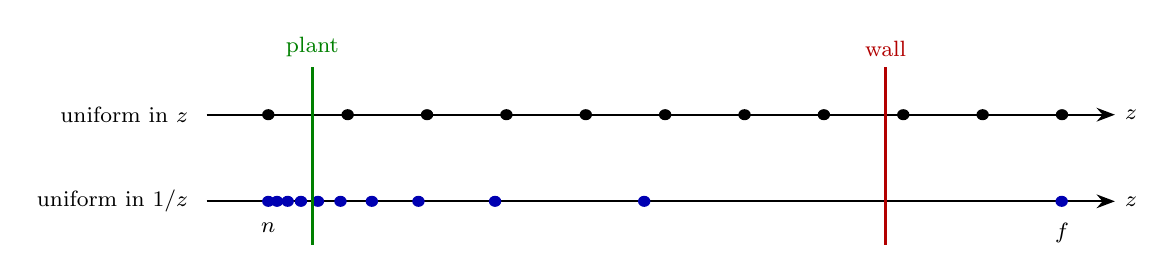
\begin{tikzpicture}[every node/.style={font=\footnotesize},xscale=1.12]
\def\near{1}
% uniform depth
\node[left] at (0.2,1.1) {uniform in $z$};
\draw[thick,-{Stealth}] (0.3,1.1)--(10.6,1.1) node[right]{$z$};
\foreach \i in {0,...,10} {\pgfmathsetmacro{\z}{1+0.9*\i}\fill (\z,1.1) circle(2pt);}
% inverse depth
\node[left] at (0.2,0) {uniform in $1/z$};
\draw[thick,-{Stealth}] (0.3,0)--(10.6,0) node[right]{$z$};
\foreach \i in {0,...,10} {\pgfmathsetmacro{\z}{1/(1-0.09*\i)}\fill[blue!70!black] (\z,0) circle(2pt);}
% objects
\draw[green!50!black,very thick] (1.5,-0.55)--(1.5,1.7) node[above]{plant};
\draw[red!70!black,very thick] (8,-0.55)--(8,1.7) node[above]{wall};
\node[below] at (1,-0.15) {$n$};\node[below] at (10,-0.15) {$f$};
\end{tikzpicture}
\caption{Original illustration, $n=1$, $f=10$, $N=10$ intervals. Uniform depth puts 8 of the 11 points beyond $z=3$; uniform inverse depth puts 7 of them within $z\le2.2$ and still reaches the far plane. The nearby plant is resolved by several samples in the second row.}
\end{figure}

\subsection{Normalised device coordinates \sref{36}}

The NeRF paper (Appendix~C) maps the depth range into $[-1,1]$ using normalised device coordinates (NDC) because real captures contain content ``anywhere between the closest point and infinity''. With near and far planes $n,f$ and camera-space depth $z_c>0$:

\begin{proposition}[NDC depth is affine in inverse depth]\label{prop:ndc}
\[
z_{\rm nd}=\frac{f+n}{f-n}-\frac{2fn}{(f-n)\,z_c}\in[-1,1].
\]
Hence sampling $z_{\rm nd}$ uniformly is the same as sampling $1/z_c$ uniformly. For $f\to\infty$, uniform inverse-depth samples are $z_i=\dfrac{n}{1-i/N}$, whereas uniform depth samples are $z_i=n+\frac iN(f-n)$.
\end{proposition}
\begin{proof}
A perspective projection yields a depth of the form $z_{\rm nd}=A+B/z_c$. The conditions $z_{\rm nd}(n)=-1$ and $z_{\rm nd}(f)=+1$ give $A+B/n=-1$ and $A+B/f=1$, so $B=\frac{2}{1/f-1/n}=-\frac{2fn}{f-n}$ and $A=1-B/f=\frac{f+n}{f-n}$. Since $z_{\rm nd}$ is affine in $1/z_c$, equal steps in $z_{\rm nd}$ are equal steps in $1/z_c$: $1/z_i=(1-s_i)/n+s_i/f$ with $s_i=i/N$; letting $f\to\infty$ gives $z_i=n/(1-s_i)$.
\end{proof}

\begin{example}
For $n=1$, $f=10$: uniform depth gives $z=1,1.9,2.8,\dots,10$; uniform inverse depth gives $z=1/(1-0.09i)=1,\,1.10,\,1.22,\,1.37,\,1.56,\,1.82,\,2.17,\,2.70,\,3.57,\,5.26,\,10$. Spacing grows steadily: the first gap is $0.10$, the last one $4.74$.
\end{example}

\begin{intuition}
A camera sees a nearby thing and a far thing at very different pixel sizes: close geometry deserves a fine depth resolution, distant geometry does not need it (it moves little on the image as the camera moves --- parallax is proportional to $1/z$). Sampling uniformly in $1/z$ spends samples proportionally to how much depth matters on the image, and lets the far plane go to infinity at the cost of one extra sample. A good detailed explanation of NDC is linked on slide~36 (\texttt{songho.ca/opengl/gl\_projectionmatrix.html}).
\end{intuition}

%==============================================================
\section{Novel-View Synthesis and View-Dependent Effects \sref{37--41}}
%==============================================================

\subsection{Novel-View Synthesis \sref{37}}

\slideimg{37}{4.6cm}{Novel-view synthesis results of NeRF on real captured scenes (a triceratops skull and a mosaic water fountain): smooth camera paths through views never seen in training. Video credits: Mildenhall et al., ECCV 2020 (NeRF).}

\subsection{View-Dependent Effects \sref{38--40}}

\begin{definition}[View-dependent effect]
A \emph{view-dependent} effect is an appearance change that results from the viewing direction alone, while geometry and light stay fixed --- specular highlights, reflections, glossy materials. In radiance-field terms: $\cc(\xx,\om_1)\neq\cc(\xx,\om_2)$ for the \emph{same} 3D point.
\end{definition}

\begin{proposition}
A representation with $\Le(\xx,\om)\equiv\cc(\xx)$ (the grid of Section~3, slide~13) cannot reproduce a scene in which the same 3D point has different colours in two training images.
\end{proposition}
\begin{proof}
By construction $\cc(\xx,\om_1)=\cc(\xx,\om_2)$; one value cannot match two different observations. The best it can do is average them, or distort the geometry (put density at wrong places) to explain the inconsistency.
\end{proof}

\begin{figure}[H]
\centering
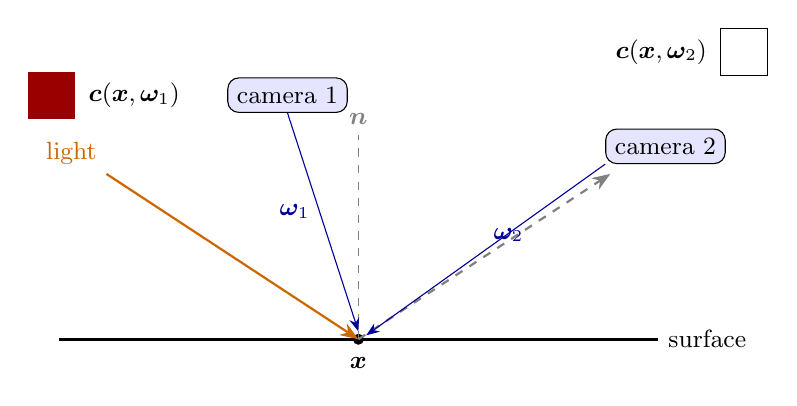
\begin{tikzpicture}[every node/.style={font=\small}]
\draw[very thick] (-3.8,0)--(3.8,0) node[right]{surface};
\fill (0,0) circle(2pt) node[below=3pt]{$\boldsymbol x$};
\draw[dashed,gray] (0,0)--(0,2.6) node[above]{$\boldsymbol n$};
% light
\draw[-{Stealth},orange!80!black,thick] (-3.2,2.1)--(0,0);
\node[orange!80!black,above left] at (-3.2,2.1) {light};
% reflection
\draw[-{Stealth},gray,dashed,thick] (0,0)--(3.2,2.1);
% cameras
\node[draw,rounded corners,fill=blue!10] (c1) at (-0.9,3.1) {camera 1};
\node[draw,rounded corners,fill=blue!10] (c2) at (3.9,2.45) {camera 2};
\draw[-{Stealth},blue!60!black] (c1.south) -- (0,0.1) node[pos=0.45,left]{$\boldsymbol\omega_1$};
\draw[-{Stealth},blue!60!black] (c2.south west) -- (0.1,0.05) node[pos=0.5,above right=-1pt]{$\boldsymbol\omega_2$};
% colour swatches
\fill[red!60!black] (-4.2,2.8) rectangle (-3.6,3.4); \node[right] at (-3.55,3.1) {$\boldsymbol c(\boldsymbol x,\boldsymbol\omega_1)$};
\fill[white,draw=black] (4.6,3.35) rectangle (5.2,3.95); \node[left] at (4.55,3.65) {$\boldsymbol c(\boldsymbol x,\boldsymbol\omega_2)$};
\end{tikzpicture}
\caption{Original illustration: a glossy surface point seen from two directions. Camera~2 lies near the mirror direction of the light and sees a bright highlight; camera~1 sees only the dark body colour. A NeRF captures this through the dependence of $\cc$ on $\om$.}
\end{figure}

\slideimg{38}{4.6cm}{Slide 38: same 3D point, different colour based on the viewing direction --- zoomed patches from two views of the synthetic ship scene (left and right) and the colour as a function of the viewing direction. Figure credits: Mildenhall et al., ECCV 2020 (NeRF).}

\slideimg{39, 40}{4.8cm}{Slides 39 and 40 (video frames): real scenes (a kitchen stove and a conference room) with highlights on metal and on the screen that move as the camera moves. Video credits: Mildenhall et al., ECCV 2020 (NeRF).}

\begin{intuition}
For a perfectly matte (Lambertian) surface, colour does not depend on the viewpoint and a grid with $\cc(\xx)$ would be enough. Real materials are not matte: the highlight on a pan slides across it when you walk around. NeRF handles it because the network gets $\om$ as input, but only in the \emph{last} layers (Proposition~\ref{prop:viewindep}): ``geometry first, appearance later''.
\end{intuition}

\subsection{Learning Neural Radiance Fields: a simple recipe \sref{41}}

Slide~41 closes the NeRF part: positional encoding at the input, a plain MLP, volume rendering and a photometric loss. It is a ``very simple'' representation and learning approach which \textbf{inspired many, many extensions and follow-ups}; the rest of the lecture visits some of them.

%==============================================================
\section{Is ray sampling accurate? \sref{42}}
%==============================================================

So far one pixel $=$ one ray through its centre. But a real pixel integrates light over a small \emph{footprint} on the sensor.

\begin{definition}[Pixel value with a box filter]
The value of pixel $\boldsymbol p$ is $I[\boldsymbol p]=\iint_{\text{pixel}}\mathrm{render}(\boldsymbol q)\dif\boldsymbol q$ (averaged over the pixel area), whereas the \emph{point-sampled} approximation uses only $\mathrm{render}(\boldsymbol p_{\rm center})$.
\end{definition}

\slideimg{42}{4.6cm}{Slide 42: a checkerboard plane rendered with one ray through each pixel centre (aliased, moir\'e pattern near the horizon) versus averaged over the whole pixel (box filter, smooth).}

\begin{figure}[H]
\centering
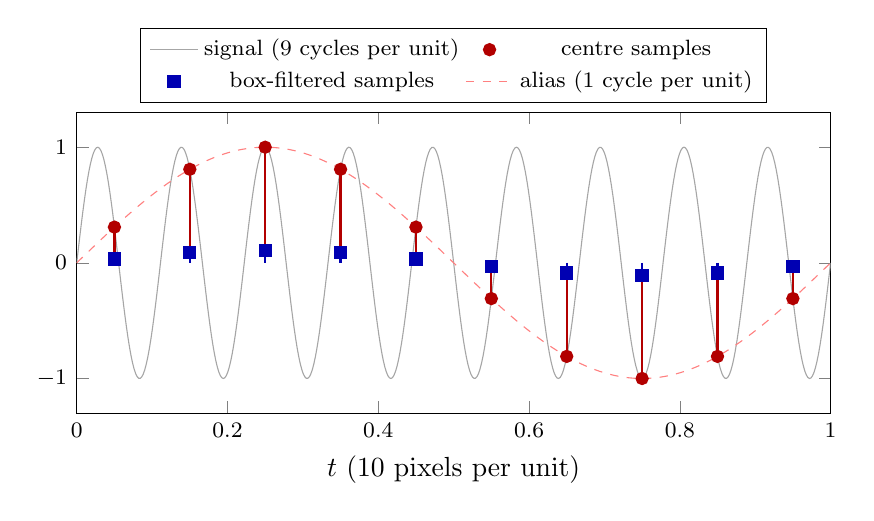
\begin{tikzpicture}
\begin{axis}[width=0.92\linewidth,height=5.4cm,xmin=0,xmax=1,ymin=-1.3,ymax=1.3,xlabel={$t$ (10 pixels per unit)},
 legend columns=2,legend style={font=\footnotesize,at={(0.5,1.03)},anchor=south},tick label style={font=\footnotesize},xtick={0,0.2,0.4,0.6,0.8,1}]
\addplot[gray!70,domain=0:1,samples=500,no markers]{sin(3240*x)};
\addplot[red!70!black,ycomb,mark=*,thick,domain=0.05:0.95,samples=10]{sin(3240*x)};
\addplot[blue!70!black,ycomb,mark=square*,thick,domain=0.05:0.95,samples=10]{0.1093*sin(3240*x)};
\addplot[red!50,dashed,domain=0:1,samples=200,no markers]{sin(360*x)};
\legend{signal (9 cycles per unit),centre samples,box-filtered samples,alias (1 cycle per unit)}
\end{axis}
\end{tikzpicture}
\caption{Original illustration of aliasing. The signal $\sin(2\pi\cdot9t)$ is far above the Nyquist limit of 5 cycles/unit for 10 pixels. Centre sampling returns a full-amplitude \emph{false} low-frequency pattern $\sin(2\pi t)$ (the moir\'e). Averaging over the pixel width $0.1$ multiplies the amplitude by $\mathrm{sinc}=\sin(0.9\pi)/(0.9\pi)\approx0.11$, so the unresolvable detail is attenuated instead of impersonating a coarse one.}
\end{figure}

\begin{intuition}
A single ray through the pixel centre answers ``what colour is the world at this exact point?'' whereas the camera asked ``what is the \emph{average} colour of this little patch?''. When the patch covers many fine details (distant checkerboard squares, or a scene viewed from far away) the two answers differ a lot. NeRF trained on images of different resolutions or distances then gets conflicting supervision from the same 3D point: sharp renders at close range look jagged/aliased, and blurry when it tries to compromise.
\end{intuition}

%==============================================================
\section{Pixels as Cones of Rays \sref{43--46}}
%==============================================================

Mip-NeRF (Barron et al., ICCV 2021) treats a pixel as a \emph{cone} (a frustum of cone between two depths $t_0,t_1$) instead of a line. Slide~43's key sentence: \emph{instead of the position encoding of a single sample, use the expected position encoding.}

\begin{figure}[H]
\centering
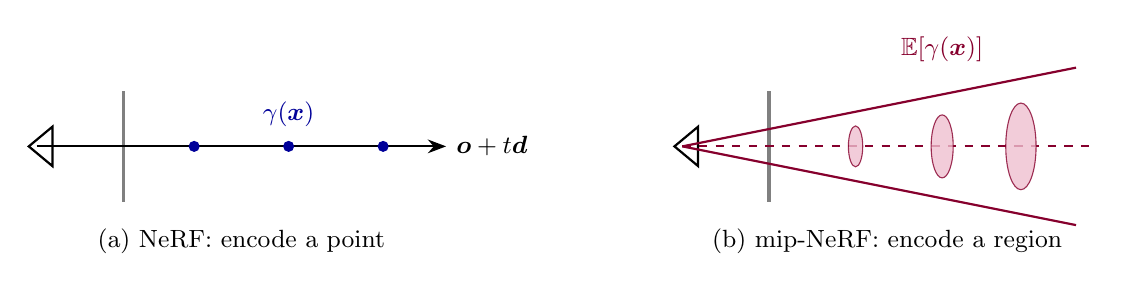
\begin{tikzpicture}[every node/.style={font=\small}]
% (a) NeRF
\begin{scope}
\draw[thick] (-0.1,0)--(0.2,0.25)--(0.2,-0.25)--cycle;
\draw[very thick,gray] (1.1,-0.7)--(1.1,0.7);
\draw[thick,-{Stealth}] (0.0,0)--(5.2,0) node[right]{$\boldsymbol o+t\boldsymbol d$};
\foreach \x in {2,3.2,4.4} {\fill[blue!60!black] (\x,0) circle(2pt);}
\node[blue!60!black,above] at (3.2,0.12) {$\gamma(\boldsymbol x)$};
\node at (2.6,-1.2) {(a) NeRF: encode a point};
\end{scope}
% (b) mip-NeRF
\begin{scope}[xshift=8.2cm]
\draw[thick] (-0.1,0)--(0.2,0.25)--(0.2,-0.25)--cycle;
\draw[very thick,gray] (1.1,-0.7)--(1.1,0.7);
\draw[thick,purple!70!black] (0.0,0)--(5.0,1.0);
\draw[thick,purple!70!black] (0.0,0)--(5.0,-1.0);
\draw[thick,dashed,purple!70!black] (0.0,0)--(5.2,0);
\foreach \x/\s in {2.2/0.26,3.3/0.4,4.3/0.55} {
  \draw[fill=purple!25,draw=purple!70!black,opacity=0.8] (\x,0) ellipse ({\s*0.35cm} and {\s*1cm});}
\node[purple!70!black,above] at (3.3,0.95) {$\E[\gamma(\boldsymbol x)]$};
\node at (2.6,-1.2) {(b) mip-NeRF: encode a region};
\end{scope}
\end{tikzpicture}
\caption{Pixels as cones of rays (redrawn from slide 43). A conical frustum covering the pixel footprint between two depths is summarised by a Gaussian with mean $\boldsymbol\mu$ and covariance $\Sigma$; the network receives the expected (integrated) positional encoding of that Gaussian. Figure credits: Barron et al., ICCV 2021 (mip-NeRF).}
\end{figure}

\begin{lemma}[Integrated positional encoding]\label{lem:ipe}
Let $X\sim\mathcal N(\mu,s^2)$ be scalar. For every frequency $a>0$,
\[
\E[\sin(aX)]=\sin(a\mu)\,e^{-a^2s^2/2},\qquad\E[\cos(aX)]=\cos(a\mu)\,e^{-a^2s^2/2}.
\]
Hence for $\boldsymbol x\sim\mathcal N(\boldsymbol\mu,\Sigma)$ coordinate-wise with $\Sigma_{jj}=s_j^2$ the expected encoding of the $k$-th band is $\sin(2^k\mu_j)\exp(-\tfrac12 4^ks_j^2)$ and $\cos(2^k\mu_j)\exp(-\tfrac12 4^ks_j^2)$.
\end{lemma}
\begin{proof}
$\E[e^{iaX}]=e^{ia\mu-a^2s^2/2}$ is the characteristic function of a Gaussian. Taking imaginary and real parts gives $\E[\sin aX]=\Im$ and $\E[\cos aX]=\Re$ of $e^{ia\mu}e^{-a^2s^2/2}$. With $a=2^k$ we have $a^2=4^k$.
\end{proof}

\begin{figure}[H]
\centering
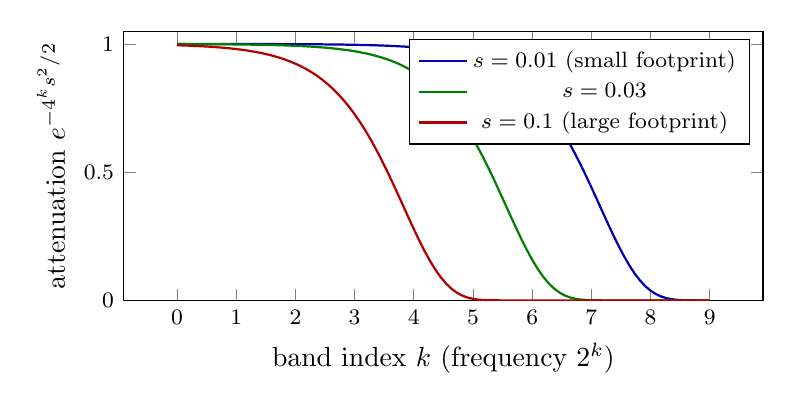
\begin{tikzpicture}
\begin{axis}[width=0.8\linewidth,height=5cm,xlabel={band index $k$ (frequency $2^k$)},ylabel={attenuation $e^{-4^ks^2/2}$},domain=0:9,samples=100,
 ymin=0,ymax=1.05,legend style={font=\footnotesize,at={(0.98,0.97)},anchor=north east},tick label style={font=\footnotesize},xtick={0,...,9}]
\addplot[blue!70!black,thick]{exp(-0.5*(2^x)^2*0.0001)};
\addplot[green!50!black,thick]{exp(-0.5*(2^x)^2*0.0009)};
\addplot[red!70!black,thick]{exp(-0.5*(2^x)^2*0.01)};
\legend{$s=0.01$ (small footprint),$s=0.03$,$s=0.1$ (large footprint)}
\end{axis}
\end{tikzpicture}
\caption{Original illustration of Lemma~\ref{lem:ipe}: the factor multiplying band $k$ of the integrated encoding. A larger footprint $s$ switches off the high-frequency bands, while a small footprint leaves them intact.}
\end{figure}

\begin{intuition}
When the pixel's footprint is large, details finer than the footprint are averaged away in the real photograph. The integrated encoding mimics this: bands whose wavelength is shorter than the footprint are smoothly \emph{damped to zero}, while coarse bands pass through untouched; the network never sees a high frequency it could not have observed. It also now knows \emph{how large} the region is, so one network can be trained on images at several resolutions. Slide~45 (mip-NeRF paper) shows that this improves the fine details at lower resolutions with the PSNR/SSIM-type numbers printed next to the crops.
\end{intuition}

\slideimg{45}{5.4cm}{Slide 45: ground truth, NeRF, NeRF + (area, centre, misc), and mip-NeRF crops of the drum and microphone scenes at several scales, with the error scores printed next to them. Figure credits: Barron et al., ICCV 2021 (mip-NeRF).}

\slideimg{46}{4.2cm}{Slide 46 (video frames): two renderings of the microphone scene compared side by side while the scale changes. Video credits: Barron et al., ICCV 2021 (mip-NeRF).}

%==============================================================
\section{Volumes: Rendering and Representation --- Option 2: An MLP, revisited \sref{47}}
%==============================================================

Slide~47 puts the MLP in perspective: it is \textbf{a very flexible representation} (continuous, compact, able to model view-dependent effects) but \textbf{can be slow to train} --- several hours for a single scene.

\begin{proposition}[Cost of one training iteration]
If a batch has $m$ rays and each ray needs $N_c+N_f$ network evaluations (Section~7), one forward--backward pass evaluates the MLP $m(N_c+N_f)$ times. 
\end{proposition}
\begin{intuition}
With e.g.\ $m=4096$ rays and $N_c+N_f=64+128=192$ samples, one iteration requires about $786{,}000$ evaluations of a 9-layer, 256-wide MLP --- and hundreds of thousands of iterations are needed. Everything that follows tries to make the \emph{query} cheaper: put the information in a grid, which only needs a few memory reads per point, instead of a deep network.
\end{intuition}

%==============================================================
\section{Option 3: Voxels with view-dependent radiance --- Do We Need Neural Radiance? \sref{48--51}}
%==============================================================

Plenoxels (Fridovich-Keil, Yu et al., CVPR 2022) answer ``\emph{do we need neural radiance?}'' with \emph{no}: keep the sparse voxel grid of Option~1 but fix its two weaknesses --- the missing view dependence and the cubic memory --- without any neural network (slide~48).

\subsection{Spherical harmonics for view-dependent colour \sref{49}}

\begin{definition}[Spherical harmonics]
The (real) spherical harmonics $Y_\ell^m:\mathbb S^2\to\R$, $\ell\ge0$, $-\ell\le m\le\ell$, are an orthonormal basis of square-integrable scalar functions on the sphere: $\int_{\mathbb S^2}Y_\ell^mY_{\ell'}^{m'}\dif\om=\delta_{\ell\ell'}\delta_{mm'}$. Degree $\ell$ contributes $2\ell+1$ functions, so truncating at degree $\ell_{\max}$ keeps $(\ell_{\max}+1)^2$ of them.
\end{definition}

\begin{definition}[View-dependent colour from basis coefficients]
Each voxel stores, for each colour channel, coefficients $k_\ell^m$ and the colour seen from direction $\om$ is
\[
\cc_{\rm ch}(\xx,\om)=\sum_{\ell\le\ell_{\max}}\sum_{m=-\ell}^{\ell}k_{\ell,{\rm ch}}^m(\xx)\,Y_\ell^m(\om)
\]
(followed in practice by a sigmoid or clamp to enforce $[0,1]$). Plenoxels uses $\ell_{\max}=2$: $9$ coefficients per channel, $27$ for RGB, plus $1$ for the density, i.e.\ $28$ numbers per voxel.
\end{definition}

\begin{lemma}[Linearity in the stored coefficients]\label{lem:sh}
The colour is a linear function of the coefficients, so trilinear interpolation of the coefficients of the eight corners and evaluation at $\om$ commutes: interpolating coefficients first and then evaluating $\sum kY$ gives the same as evaluating each corner's colour first and then interpolating. Moreover $\partial\cc_{\rm ch}/\partial k_\ell^m=Y_\ell^m(\om)$ (times the interpolation weight).
\end{lemma}
\begin{proof}
Both operations are linear combinations of the corner coefficients with weights $\lambda_{ijk}$ (Lemma~\ref{lem:trilin}) and $Y_\ell^m(\om)$, which do not depend on one another. The derivative is read off the formula.
\end{proof}

\begin{figure}[H]
\centering
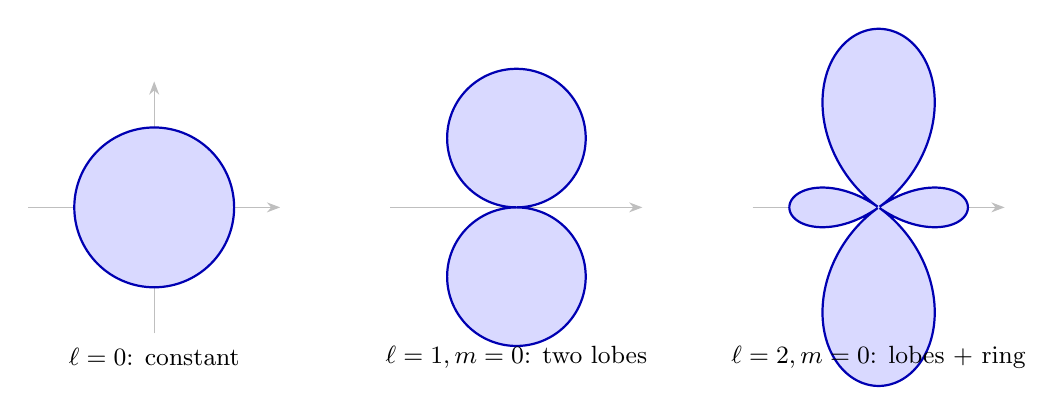
\begin{tikzpicture}[every node/.style={font=\small},scale=1.0]
% l=0
\begin{scope}
\draw[gray!50,-{Stealth}] (-1.6,0)--(1.6,0); \draw[gray!50,-{Stealth}] (0,-1.6)--(0,1.6);
\draw[blue!70!black,thick,fill=blue!15] plot[domain=0:360,samples=121,smooth cycle] ({1.015*sin(\x)},{1.015*cos(\x)});
\node at (0,-1.9) {$\ell=0$: constant};
\end{scope}
% l=1
\begin{scope}[xshift=4.6cm]
\draw[gray!50,-{Stealth}] (-1.6,0)--(1.6,0); \draw[gray!50,-{Stealth}] (0,-1.6)--(0,1.6);
\draw[blue!70!black,thick,fill=blue!15] plot[domain=0:360,samples=181,smooth cycle] ({1.76*abs(cos(\x))*sin(\x)},{1.76*abs(cos(\x))*cos(\x)});
\node at (0,-1.9) {$\ell=1,m=0$: two lobes};
\end{scope}
% l=2
\begin{scope}[xshift=9.2cm]
\draw[gray!50,-{Stealth}] (-1.6,0)--(1.6,0); \draw[gray!50,-{Stealth}] (0,-1.6)--(0,1.6);
\draw[blue!70!black,thick,fill=blue!15] plot[domain=0:360,samples=361,smooth cycle] ({1.134*abs(3*cos(\x)*cos(\x)-1)*sin(\x)},{1.134*abs(3*cos(\x)*cos(\x)-1)*cos(\x)});
\node at (0,-1.9) {$\ell=2,m=0$: lobes + ring};
\end{scope}
\end{tikzpicture}
\caption{Original illustration (slide 49 shows the full pyramid of harmonics): polar plots of the magnitude $|Y_\ell^0(\theta)|$ of the zonal harmonics for $\ell=0,1,2$ (vertical axis = polar axis; lobes alternate in sign). Higher degrees add angular detail, i.e.\ faster variation of colour with the viewing direction.}
\end{figure}

\begin{intuition}
Spherical harmonics are the Fourier series of the sphere. The $\ell=0$ coefficient is the average, view-independent colour (the ``diffuse'' part); $\ell=1$ lets the colour tilt towards one side of the sphere, and $\ell=2$ adds richer variation like highlight shapes. Storing a handful of coefficients per voxel is therefore a compact table of \emph{how the colour of this voxel changes around the sphere}, so the voxel no longer has the single colour of Option~1 --- exactly the missing ingredient in slide~17 ---, and no network is needed to get it.
\end{intuition}

\subsection{The Plenoxels pipeline \sref{50}}

\begin{algorithm}[Plenoxels, slide 50]\label{alg:plenox}
\begin{enumerate}[nosep]
\item \textbf{Sparse voxel grid.} At each voxel store the density and the spherical-harmonic coefficients for view-dependent colour.
\item \textbf{Trilinear interpolation} of density and coefficients at every sample along the ray (Lemma~\ref{lem:trilin}); evaluate $Y_\ell^m(\om)$ to get the colour.
\item \textbf{Volumetric rendering} (Theorem~\ref{thm:render}) to obtain the predicted colour.
\item \textbf{Optimisation:} minimise $\mathcal L_{\rm recon}+\lambda\mathcal L_{TV}$ over all voxel values directly by gradient descent.
\item For efficiency, \textbf{prune voxels with very low density} (they carry no visible information).
\end{enumerate}
\end{algorithm}

Here $\mathcal L_{\rm recon}$ is the same photometric loss as for NeRF and $\mathcal L_{TV}$ a total-variation regulariser, which penalises large differences between neighbouring voxels, e.g.\ $\mathcal L_{TV}\propto\sum_{v}\sum_{d\in\{x,y,z\}}|\,f(v)-f(v+e_d)\,|$ for each stored quantity $f$.

\begin{figure}[H]
\centering
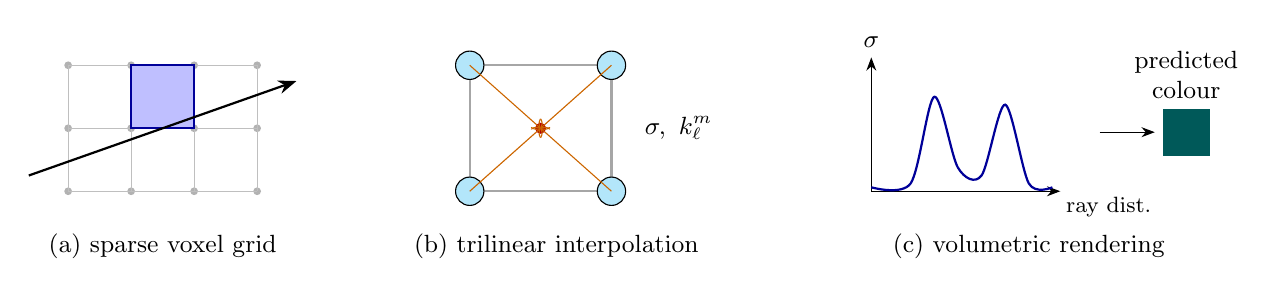
\begin{tikzpicture}[every node/.style={font=\small}]
% (a) sparse voxel grid
\begin{scope}
\foreach \i in {0,...,3} \foreach \j in {0,...,2} {\fill[gray!60] (0.8*\i,0.8*\j) circle(1.4pt);}
\draw[gray!50] (0,0) grid[step=0.8] (2.4,1.6);
\fill[blue!25] (0.8,0.8) rectangle (1.6,1.6);
\draw[blue!60!black,thick] (0.8,0.8) rectangle (1.6,1.6);
\draw[-{Stealth},thick] (-0.5,0.2)--(2.9,1.4);
\node at (1.2,-0.7) {(a) sparse voxel grid};
\end{scope}
% (b) interpolation in a cell
\begin{scope}[xshift=5.1cm]
\draw[gray!70,thick] (0,0) rectangle (1.8,1.6);
\foreach \x/\y in {0/0,1.8/0,0/1.6,1.8/1.6} {\draw[fill=cyan!30] (\x,\y) circle(0.18);}
\fill[red!70!black] (0.9,0.8) circle(2pt);
\foreach \x/\y in {0/0,1.8/0,0/1.6,1.8/1.6} {\draw[->,orange!80!black] (\x,\y)--(0.9,0.8);}
\node[right] at (2.1,0.8) {$\sigma,\ k_\ell^m$};
\node at (1.1,-0.7) {(b) trilinear interpolation};
\end{scope}
% (c) rendering
\begin{scope}[xshift=10.2cm]
\draw[-{Stealth}] (0,0)--(2.4,0) node[below right=-2pt]{\footnotesize ray dist.};
\draw[-{Stealth}] (0,0)--(0,1.7) node[above]{$\sigma$};
\draw[blue!60!black,thick] plot[smooth] coordinates {(0,0.05)(0.5,0.1)(0.8,1.2)(1.1,0.3)(1.4,0.2)(1.7,1.1)(2.0,0.1)(2.3,0.05)};
\fill[teal!70!black] (3.7,0.45) rectangle (4.3,1.05);
\node[above,align=center] at (4.0,1.05) {predicted\\ colour};
\draw[-{Stealth}] (2.9,0.75)--(3.6,0.75);
\node at (2.0,-0.7) {(c) volumetric rendering};
\end{scope}
\end{tikzpicture}
\caption{The Plenoxels pipeline (redrawn from slide 50; original figure by Fridovich-Keil, Yu et al., CVPR 2022): (a) sparse voxel grid; (b) trilinear interpolation of the eight corner values; (c) volumetric rendering along the ray; (d, not drawn) optimisation of the voxel values with $\mathcal L_{\rm recon}+\lambda\mathcal L_{TV}$.}
\end{figure}

\begin{intuition}
There is nothing to ``forward'' through a network: a query is eight memory reads and a few multiplications, and the gradient w.r.t.\ a voxel value is just its interpolation weight (Lemma~\ref{lem:trilin}(iv)). That is why training takes minutes rather than hours. The price is more memory (28 numbers per voxel) and some noise when views are few, which TV smoothing fights.
\end{intuition}

\subsection{NeRF vs.\ Plenoxels \sref{51}}

\slideimg{51}{4.8cm}{Slide 51 (video frames): training NeRF (left) and Plenoxels (right) side by side with a \texttt{minutes:seconds} timer; Plenoxels reaches a recognisable result long before NeRF. Figure credits: Fridovich-Keil, Yu et al., CVPR 2022 (Plenoxels).}

%==============================================================
\section{Towards Hybrid Representations \sref{52--54}}
%==============================================================

\emph{Option 4: feature hash-grid $+$ lightweight MLP} (Instant-NGP, M\"uller et al., SIGGRAPH 2022). The idea combines the two worlds: store \emph{learned features} in a (hashed) grid for fast lookups, and let a \emph{tiny} MLP map those features and the direction to density and colour (slide~53).

\begin{definition}[Multiresolution hash encoding]\label{def:hash}
Use $L$ resolution levels, with grid resolutions $N_\ell=\lfloor N_{\min}\,b^{\ell}\rfloor$ (geometric growth factor $b$). Level $\ell$ owns a table $\theta_\ell\in\R^{T\times F}$ of $T$ entries with $F$ features each. For $\xx\in[0,1]^d$:
\begin{enumerate}[nosep]
\item \emph{Hashing of voxel vertices:} the $2^d$ integer vertices $\boldsymbol c$ of the cell containing $\xx N_\ell$ are mapped to table slots by $h(\boldsymbol c)=\big(\bigoplus_{i=1}^dc_i\pi_i\big)\bmod T$, with large primes $\pi_i$ ($\pi_1=1$, $\pi_2=2654435761$, $\pi_3=805459861$ in the paper) and $\oplus$ the bitwise XOR. If the level has at most $T$ vertices it is indexed directly.
\item \emph{Lookup} of the $F$-dimensional features of the vertices.
\item \emph{(Multi)linear interpolation} of those features with the weights of Lemma~\ref{lem:trilin} (the 2D version for $d=2$ in the slide).
\item \emph{Concatenation} of the $L$ interpolated vectors (giving $L\cdot F$ numbers) with auxiliary inputs $\xi$ (e.g.\ the encoded view direction): $\boldsymbol y\in\R^{LF+E}$.
\item \emph{Neural network:} a tiny MLP $m(\boldsymbol y;\Phi)$ outputs density and colour.
\end{enumerate}
\end{definition}

\begin{figure}[H]
\centering
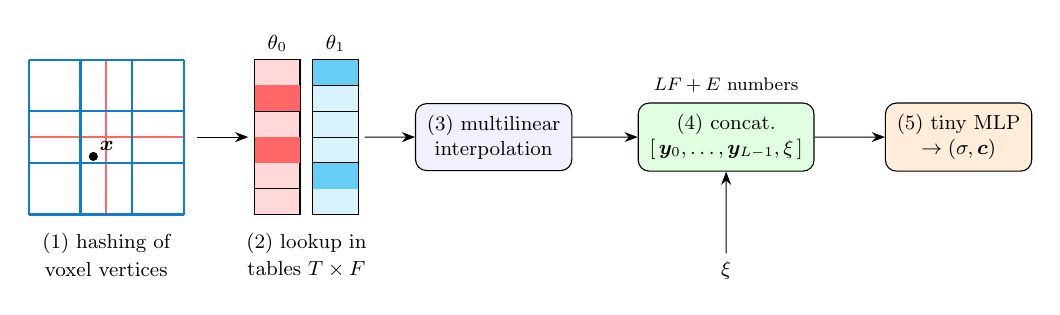
\begin{tikzpicture}[every node/.style={font=\small},scale=0.82,transform shape,box/.style={draw,rounded corners,align=center,inner sep=5pt,fill=blue!6}]
% grids
\begin{scope}
\draw[red!60,thick] (0,0) grid[step=1.2] (2.4,2.4);
\draw[cyan!60!blue,thick] (0,0) grid[step=0.8] (2.4,2.4);
\fill (1.0,0.9) circle(2pt) node[above right=-1pt]{$\boldsymbol x$};
\node at (1.2,-0.45) {(1) hashing of};
\node at (1.2,-0.85) {voxel vertices};
\end{scope}
% tables
\begin{scope}[xshift=3.5cm]
\foreach \i in {0,...,5} {\draw[fill=red!15] (0,2.4-0.4*\i-0.4) rectangle (0.7,2.4-0.4*\i);}
\foreach \i in {0,...,5} {\draw[fill=cyan!15] (0.9,2.4-0.4*\i-0.4) rectangle (1.6,2.4-0.4*\i);}
\foreach \i in {1,3} {\fill[red!60] (0,2.4-0.4*\i-0.4) rectangle (0.7,2.4-0.4*\i);}
\foreach \i in {0,4} {\fill[cyan!60] (0.9,2.4-0.4*\i-0.4) rectangle (1.6,2.4-0.4*\i);}
\node at (0.35,2.65) {$\theta_0$}; \node at (1.25,2.65) {$\theta_1$};
\node at (0.8,-0.45) {(2) lookup in};\node at (0.8,-0.85) {tables $T\times F$};
\end{scope}
\draw[-{Stealth}] (2.6,1.2)--(3.4,1.2);
% interp
\node[box] (it) at (7.2,1.2) {(3) multilinear\\ interpolation};
\draw[-{Stealth}] (5.2,1.2)--(it.west);
% concat
\node[box,fill=green!12] (cc) at (10.8,1.2) {(4) concat.\\ $[\,\boldsymbol y_0,\dots,\boldsymbol y_{L-1},\xi\,]$};
\draw[-{Stealth}] (it)--(cc);
\node[above=1pt of cc,font=\footnotesize] {$LF+E$ numbers};
% mlp
\node[box,fill=orange!15] (mlp) at (14.4,1.2) {(5) tiny MLP\\ $\to(\sigma,\boldsymbol c)$};
\draw[-{Stealth}] (cc)--(mlp);
\draw[-{Stealth}] (10.8,-0.6)--(cc.south) node[pos=0,below]{$\xi$};
\end{tikzpicture}
\caption{The hash-grid encoding (redrawn from slides 52--53; original figure by M\"uller et al., SIGGRAPH 2022). Two levels of a 2D toy grid are shown. Each level has its own small table; vertices from many places of space can share a table slot (hash collision).}
\end{figure}

\begin{proposition}[Memory is fixed by the hyper-parameters, not by the scene]\label{prop:hashmem}
The encoding has $L\cdot T\cdot F$ trainable numbers regardless of the resolution $N_L$ reached by the finest level, whereas a dense grid of the same finest resolution needs $(N_L+1)^d$ vertices.
\end{proposition}
\begin{intuition}
Example with the typical NeRF-style values $L=16$, $F=2$, $T=2^{19}$ (as reported for Instant-NGP): $16\cdot524{,}288\cdot2\approx16.8$M numbers --- about $34$~MB in half precision --- whether the finest resolution is $512$ or $2048$ per axis; a dense $2048^3$ grid with 4 values per voxel in single precision would need $\approx137$~GB. How do we get away with this? Real scenes are mostly empty: only $\sim N^2$ vertices near surfaces matter, which is of the order of the table size, and when two vertices collide the network and the gradients (dominated by the vertex that matters more for the image) sort it out; the coarse levels have no collisions and give context. The tiny MLP (e.g.\ 1--2 hidden layers of 64 units in the paper) is cheap because the features already carry the spatial information.
\end{intuition}

\begin{figure}[H]
\centering
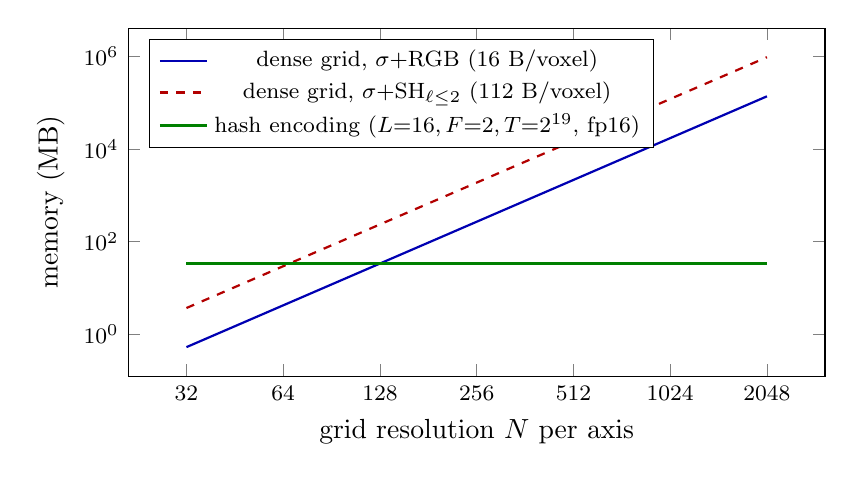
\begin{tikzpicture}
\begin{axis}[width=0.86\linewidth,height=6cm,xmode=log,ymode=log,log basis x=2,xlabel={grid resolution $N$ per axis},ylabel={memory (MB)},domain=32:2048,samples=40,
  legend style={font=\footnotesize,at={(0.03,0.97)},anchor=north west},tick label style={font=\footnotesize},
  xtick={32,64,128,256,512,1024,2048},xticklabels={32,64,128,256,512,1024,2048}]
\addplot[blue!70!black,thick]{x^3*16/1e6};
\addplot[red!70!black,thick,dashed]{x^3*112/1e6};
\addplot[green!50!black,very thick]{33.5};
\legend{{dense grid, $\sigma+$RGB (16 B/voxel)},{dense grid, $\sigma+$SH$_{\ell\le2}$ (112 B/voxel)},{hash encoding ($L{=}16,F{=}2,T{=}2^{19}$, fp16)}}
\end{axis}
\end{tikzpicture}
\caption{Original illustration: memory of dense grids grows as $N^3$ (a straight line of slope 3 on this log-log plot) while the hash encoding stays constant (assumed values $L=16$, $F=2$, $T=2^{19}$, half precision). Plenoxels avoids most of the dense cost by storing only occupied voxels (sparse grid), so its real footprint is much smaller than the dashed line.}
\end{figure}

\slideimg{54}{4.8cm}{Slide 54 (video frames): Instant-NGP training on eight different scenes/images with an ``Elapsed training time'' counter --- a usable result appears after seconds. Video credits: M\"uller et al., SIGGRAPH 2022 (Instant-NGP).}

\textbf{Remark.} Slide~53 notes that the core idea --- a hash function that efficiently stores per-voxel features, plus a tiny MLP that maps a query point's features (and direction) to colour and density --- is applicable to the efficient modelling of general 2D/3D signals, not only radiance fields (images, signed distance functions, \dots).

%==============================================================
\section{Summary \sref{55}}
%==============================================================

Slide~55: \emph{last lecture}: volume rendering; \emph{today}: neural representations for volumes, and training via view synthesis. The common recipe is: (representation of $\sigma,\Le$) $\to$ differentiable ray marching $\to$ photometric loss with posed images.

\slideimg{55}{4.4cm}{Slide 55: training images $\to$ MLP / sparse voxel grid with spherical harmonics $\to$ novel view of the lego scene. Figure credits: Mildenhall et al. (NeRF), Fridovich-Keil, Yu et al. (Plenoxels).}

\begin{table}[htbp]
\centering
\footnotesize
\setlength{\tabcolsep}{3pt}
\renewcommand{\arraystretch}{1.25}
\begin{tabular}{@{}>{\raggedright\arraybackslash}p{1.9cm}>{\raggedright\arraybackslash}p{2.9cm}>{\raggedright\arraybackslash}p{2.0cm}>{\raggedright\arraybackslash}p{3.3cm}>{\raggedright\arraybackslash}p{2.0cm}>{\raggedright\arraybackslash}p{2.7cm}@{}}
\toprule
\textbf{Method} & \textbf{Representation} & \textbf{View-dep. colour} & \textbf{Key idea} & \textbf{Training time (slides)} & \textbf{Main limitation}\\
\midrule
Voxel grid (Opt.~1) & $\sigma[x,y,z]$, $\cc[x,y,z]$, trilinear interp. & No ($\Le\equiv\cc(\xx)$) & Store values on a lattice; differentiable lookups & fast queries & cubic memory; no view effects\\
\addlinespace
NeRF (Opt.~2) & MLP $f_\theta(\xx,\om)\to(\sigma,\cc)$ & Yes, $\om$ injected late & Photometric loss through volume rendering; positional encoding; hierarchical sampling & several hours per scene & slow to train; blurry without $\gamma$\\
\addlinespace
mip-NeRF & NeRF with cones and integrated encoding $\E[\gamma(\xx)]$ & Yes & Pixels are footprints, not points; anti-aliasing across scales & like NeRF & still an MLP: slow\\
\addlinespace
Plenoxels (Opt.~3) & sparse voxels: $\sigma$ + SH coefficients & Yes (spherical harmonics) & No network; optimise voxels directly with $\mathcal L_{\rm recon}+\lambda\mathcal L_{TV}$; prune empty voxels & minutes & large memory per voxel ($28$ numbers); noise with few views\\
\addlinespace
Instant-NGP (Opt.~4) & multires hash-grid features $+$ tiny MLP & Yes (direction goes into the MLP) & Fixed-size learned hash tables; tiny MLP & seconds to minutes & hash collisions; fixed table size\\
\bottomrule
\end{tabular}
\caption{Comparison of the representations seen in the lecture. All share the same rendering equation (Theorem~\ref{thm:render}) and photometric training signal; they differ in how $\sigma(\xx)$ and $\Le(\xx,\om)$ are stored and queried.}
\end{table}

\begin{figure}[H]
\centering
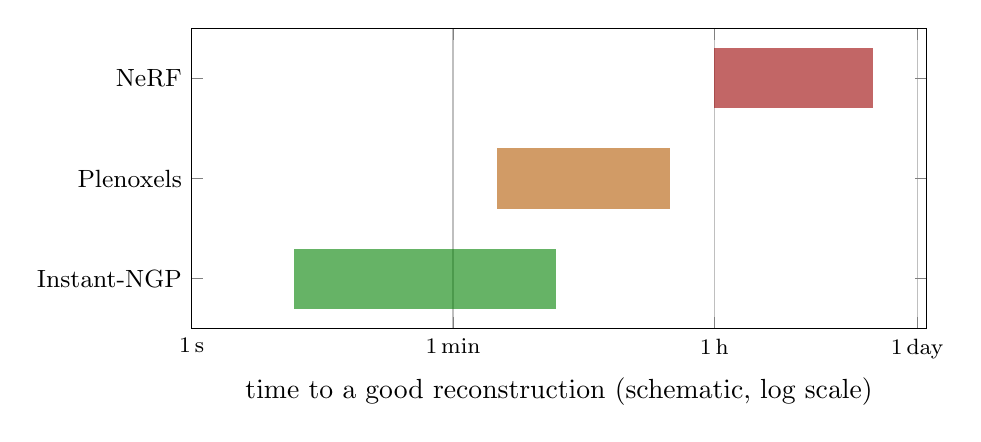
\begin{tikzpicture}
\begin{axis}[width=0.9\linewidth,height=5.4cm,xmode=log,xmin=1,xmax=1e5,ymin=0,ymax=3,
  xtick={1,60,3600,86400},xticklabels={1\,s,1\,min,1\,h,1\,day},ytick={0.5,1.5,2.5},yticklabels={Instant-NGP,Plenoxels,NeRF},
  xlabel={time to a good reconstruction (schematic, log scale)},tick label style={font=\footnotesize},y tick label style={font=\small},
  xmajorgrids,minor tick num=0]
\fill[green!50!black,opacity=0.6] (axis cs:5,0.2) rectangle (axis cs:300,0.8);
\fill[orange!70!black,opacity=0.6] (axis cs:120,1.2) rectangle (axis cs:1800,1.8);
\fill[red!60!black,opacity=0.6] (axis cs:3600,2.2) rectangle (axis cs:43200,2.8);
\end{axis}
\end{tikzpicture}
\caption{Qualitative comparison (schematic, orders of magnitude only; not measured here): the slides only state ``several hours'' for NeRF, and show timers of minutes for Plenoxels and seconds for Instant-NGP. Moving information from deep networks into explicit/hashed grids buys one to three orders of magnitude in training time.}
\end{figure}

\subsection*{Key take-aways}
\begin{itemize}
\item \textbf{Volume rendering is the differentiable bridge.} Density and emitted light along a ray give a pixel via $L=\sum_iT_i(1-e^{-\sigma_i\Delta t_i})\cc_i$ (+ background $T_{N+1}L_{\rm bg}$), with weights summing to one; gradients flow to densities, colours and, if these are differentiable functions of position and direction, to the camera.
\item \textbf{A radiance field is any function $(\xx,\om)\mapsto(\sigma,\cc)$.} It can be a grid (fast but cubic memory, no view effects), an MLP (compact, flexible, slow), voxels with spherical harmonics, or a hash-grid with a tiny MLP; training is always ``match the posed images'' (view synthesis loss on randomly sampled rays).
\item \textbf{Details make or break NeRF:} positional encoding $\gamma$ overcomes spectral bias; density depends on $\xx$ only while colour also on $\om$; hierarchical (importance) sampling spends queries where $w_i$ is large; inverse-depth/NDC sampling handles unbounded scenes.
\item \textbf{Pixels are areas, not points:} mip-NeRF replaces the encoding of a single point by the expected (integrated) encoding of the pixel's conical frustum, which damps frequencies finer than the footprint and removes aliasing.
\item \textbf{Hybrid representations trade neural computation for memory lookups:} sparse voxels + SH (Plenoxels) and multiresolution hash features + tiny MLP (Instant-NGP) reduce training from hours to minutes or seconds.
\end{itemize}

\vfill
\small\textit{Credits.} Slides adapted from \emph{Learning for 3D Vision}, CMU 16-825 (Prof.\ Shubham Tulsiani). Ray-marching figures by Ioannis (Yannis) Gkioulekas. Results and diagrams from Mildenhall et al., ECCV 2020 (NeRF); Tancik et al., NeurIPS 2020 (Fourier Features); Barron et al., ICCV 2021 (mip-NeRF); Fridovich-Keil, Yu et al., CVPR 2022 (Plenoxels); M\"uller et al., SIGGRAPH 2022 (Instant-NGP).

\end{document}